% LaTeX-Vorlage zur Erstellung einer Abschlussarbeit in der Fakultät Elektrotechnik, Medien und Informatik an der OTH Amberg-Weiden
% Diese Vorlage entstand im Rahmen des Kurses "LaTeX fürs Studium"
% Aktuelle Version: v0.03bacsem
% Stand: 18.04.2020
%
% Changelog:
%
% v0.03bacsem-us: 28.04.2020, Grafikpfad und Bibliographiemanagement 
%                             via bibtex hinzugefügt
% Grafikpfad für das graphicx-Paket:
%   \graphicspath{{images/}} % hinter \usepackage{graphicx}
% Literaturverzeichnis nach DIN:          
%   \usepackage[square,numbers,sort]{natbib} 
% Literaturverzeichnis am Ende:
%   \bibliographystyle{natdin}
%   \bibliography{literatur}
% 
% v0.02: 06.08.2015, Anpassung der Vorlage:
% + Persönliche Informationen (Vorname, Name, Titel usw.) werden direkt in die PDF-Dokumenteinstellungen übernommen
% + Korrektur der Verlinkung von Abbildungs- und Tabellenverzeichnis aus dem Inhaltsverzeichnis (phantomsection) bzw. deren Seitenzahl
%   Besten Dank für diesen Hinweis an Jan-Olaf Becker
% + Anpassung des Namens der Fakultät nach deren Umbenennung
%
% v0.01: 14.03.2012, Erstellung der Vorlage
% oneside: legt Seitennummerierung in die Mitte -> einseitiger Druck
% twoside: legt Seitennummerierung abh. von Seite an rechten/linken Rand -> vorder-/rueckseite Druck
\documentclass[12pt,oneside]{report}
\usepackage[T1]{fontenc}		% Einstellungen fuer Umlaute usw.
\usepackage[utf8x]{inputenc}
\usepackage[ngerman]{babel}

\usepackage{parskip}			% Einstellungen fuer Absaetze: Abstand statt Einrueckung

\usepackage[a4paper,			% Papierformat A4
	    left=2.0cm,				% linker Rand
	    right=2.0cm,			% rechter Rand
	    top=2.0cm,				% oberer Rand
	    bottom=2.0cm,			% unter Rand
	    marginparsep=5mm,		% Abstand der Randnotizen
	    marginparwidth=10mm, 	% Breite der Randnotizen
	    headheight=7mm,			% Hoehe der Kopfzeile
	    headsep=1.2cm,			% Abstand der Kopfzeile
	    footskip=1.5cm,			% Abstand der Fusszeile
	    includeheadfoot]{geometry}

\usepackage{fancyhdr}						% Konfiguration von Kopf- und Fusszeilen
\pagestyle{fancy}							% Seitenstil 'fancy'
\fancyhf{}									% vorhandene Einstellungen loeschen
\setlength{\headwidth}{\textwidth}			% Kopf- und Fusszeile so breit wie der Haupttext
\fancyfoot[R]{\thepage} 					% Festlegung des Seitenstils: Seitenzahlen in der Fusszeile rechts
\fancyfoot[L]{\leftmark}					% Kapitelnr. und -Bezeichnung in der Fusszeile links
\fancyhead[R]{\IhreArbeit}					% "Bachelorarbeit" in der Kopfzeile rechts
\fancyhead[L]{\IhrVorname\ \IhrNachname}	% Vorname und Name in der Kopfzeile links
\renewcommand{\chaptermark}[1]{			% Definition der Ausgabe des Kapitels
  \markboth{Kapitel \thechapter. #1}{}}
\renewcommand{\headrulewidth}{0.5pt}		% Trennlinie zwischen Kopfzeile und Haupttext
\renewcommand{\footrulewidth}{0.5pt}		% Trennlinie zwischen Haupttext und Fusszeile
\fancypagestyle{plain}{					% Anpassung des Seitenstils 'plain' bei Beginn neuer Kapitel
  \fancyhf{}								% Vorbelegung loeschen
  \fancyfoot[C]{\thepage}					% Seitenzeilen in der Fusszeile mittig
  \fancyhead[R]{\IhreArbeit}				% "Bachelorarbeit" in der Kopfzeile rechts
  \fancyhead[L]{\IhrVorname\ \IhrNachname}	% Vorname und Name in der Kopfzeile links
}

%\usepackage{amsmath}			% Pakete fuer den Mathematikmodus
%\usepackage{amssymb}
\usepackage[intlimits]{empheq}

\usepackage[sc]{mathpazo}		% Schriftart Palatino fuer Haupttext und Mathematikmodus
\usepackage{pifont}				% zusaetzliche Symbole

\usepackage{setspace}
\setstretch{1.25}

\usepackage[format=hang,		% Einstellung fuer Bildunterschriften
            font={footnotesize},
            labelfont={bf},
            margin=1cm,
            aboveskip=5pt,
            position=bottom]{caption}

\usepackage{graphicx}	   % Einbinden von Grafiken (jpg, png, pdf, ...)
\graphicspath{{images/}}   % Suchpfad für Grafikdateien

\usepackage[svgnames,table,hyperref]{xcolor} 	% Verwendung von Farben
\usepackage{tikz}								% Erstellen von Grafiken
\usetikzlibrary{positioning,arrows,plotmarks} % TikZ-Bibliotheken
%\usepackage{pgfplots}                           % Darstellung von Plots, Funktionen, Graphen usw.

%
% Weitere Pakete
%
\usepackage{listings}			% Darstellung von Quellcode
\definecolor{mygreen}{rgb}{0,0.6,0}
\definecolor{myblue}{rgb}{0.0,0.0,1.0}
\definecolor{myred}{rgb}{1.0,0.3,0.0}

\DeclareMathOperator{\arctantwo}{arctan2}

\usepackage{leftidx}

\lstset{language = Python,
	numbers = none,
	basicstyle = \small\ttfamily,
	keywordstyle = \color{myblue},
	commentstyle = \color{mygreen},
	stringstyle = \color{myred},
	columns = flexible,
	showstringspaces = false,
	frame = single,
	morekeywords={as, family}
}
\usepackage{float}
\usepackage[square,numbers,sort]{natbib} % Referenzen
%
%\usepackage[european, siunitx]{circuitikz}	% Darstellung von Schaltungen
%
%\usepackage{enumerate}			% Formatierung nummerierter Listen

\usepackage{microtype,relsize}					% Wird verwendet, um Nachnamen auf Titelseite gesperrt darzustellen
\newcommand*{\Sperren}[1]{\textls*[100]{#1}}

% 
% Persoenliche Angaben
% 
\newcommand*{\IhrVorname}{André}
\newcommand*{\IhrNachname}{Kestler}
\newcommand*{\IhrStudiengang}{Künstliche Intelligenz}
% Bachelorarbeit, Masterarbeit, Studienarbeit
\newcommand*{\IhreArbeit}{Studienarbeit Deep Vision}
\newcommand*{\IhrTitelDE}{Vergleich der YOLOX- und YOLOv8-Modelle für die Objekterkennung im Kontext des Udacity Self Driving Car-Datensatzes}
\newcommand*{\IhrBearbeitungszeitraumVON}{21. Juni 2023}
\newcommand*{\IhrBearbeitungszeitraumBIS}{19. Juli 2023}
\newcommand*{\IhrErstpruefer}{Prof. Dr. phil. Tatyana Ivanovska}


\usepackage[bookmarks, raiselinks, pageanchor, % PDF-Einstellungen
            hyperindex, colorlinks,
            citecolor=black, linkcolor=black,
            urlcolor=black, filecolor=black,
            menucolor=black]{hyperref}
\hypersetup{pdftitle={\IhrTitelDE},%
            pdfauthor={\IhrVorname\ \IhrNachname},%
            pdfsubject={\IhreArbeit}}

\usepackage{subcaption} 
\usepackage{array}
%
% Beginn des Textteils
%
\begin{document}
    \pagenumbering{roman}
  \thispagestyle{empty}
  \begin{center}
    \Large
    Ostbayerische Technische Hochschule Amberg-Weiden\\
    Fakultät Elektrotechnik, Medien und Informatik\\[1cm]
    Studiengang \IhrStudiengang\\[1cm]
    \textbf{\IhreArbeit}\\[1cm]
    von\\[1cm]
    \IhrVorname\ \Sperren{\textbf{\IhrNachname}}\\[1cm]
    \textbf{\IhrTitelDE}\\[1cm]
%    \IhrTitelE
  \end{center}
  \vspace*{2.5cm}
  \begin{tabbing}
    \underbar{Bearbeitungszeitraum:}\qquad\= von\qquad\=\IhrBearbeitungszeitraumVON\\
                                          \> bis      \>\IhrBearbeitungszeitraumBIS
  \end{tabbing}
  \vspace*{1cm}
  \underbar{1. Prüfer:}\qquad\IhrErstpruefer\par 
 % \underbar{2. Prüfer:}\qquad\IhrZweitpruefer
    \tableofcontents
    \thispagestyle{empty}
 	\newpage
  
% ----------------------------------------------------------------------  
  
%  \chapter*{Symbole, Formelzeichen und Einheiten}
 % \begin{tabular}{ll}
 % 	%$I$ & Einheitsmatrix\\
 % 	%GB     & Gigabyte ($10^9$ Bytes)\\
 % \end{tabular}
 % \newpage
  
% ----------------------------------------------------------------------  
  \chapter*{Abkürzungsverzeichnis}
    \begin{tabular}{ll}
    	%KI	& Künstliche Intelligenz\\
    	CSPDarknet & Cross Stage Partial Network Darknet\\
    	FPN & Feature Pyramide Network\\
    	IoU & Intersection over Union\\
    	OTA & Optimal Transport Assignment\\
    	PAFPN & Path Aggregation Feature Pyramid Network (Kombination von FPN und PAN)\\
    	PAN & Path Aggregation Network\\
    	SPP & Spartial Pyramid Pooling\\
    	YOLO & You only look once\\
  	\end{tabular}

  \newpage
  \pagenumbering{arabic}
  % Kapitel einfügen
  
  \chapter{Einleitung}

\section{Aufgabenstellung}
Im Rahmen der Vorlesung Deep Vision ist ein Projekt im Themenbereich des Kurses zu bearbeiten. Die Bearbeitung erfolgt als Einzelarbeit. Als Projekt werden zwei YOLO (You only look once) Netzwerke mit dem Udacity Self Driving Car Datensatz trainiert und miteinander verglichen. In der folgenden Arbeit werden YOLOX und YOLOv8 verwendet.


\section{Übersicht}
In Kapitel \ref{chap:dataset} wird zunächst der Datensatz beschrieben. Dabei wird auf die Klasseneinteilung und die Datenstruktur eingegangen. In Kapitel \ref{chap:yolox} wird das YOLOX-Netzwerk vorgestellt. Dabei wird auf die verwendete Verlustfunktion, die Architektur und die Ergebnisse mit dem Datensatz eingegangen. Kapitel \ref{chap:yolov8} beschreibt die verwendete Architektur von YOLOv8. Außerdem werden die Ergebnisse anhand des verwendeten Datensatzes präsentiert. Das letzte Kapitel befasst sich mit dem direkten Vergleich der Ergebnisse und gibt einen Ausblick über die weitere Bearbeitung. Im \nameref{chap:appendix} wird beschrieben, wie die angegebenen Skripte verwendet werden, um die Netzwerke selbst zu trainieren.



  % Hauptteil
  \chapter{Datensatz}\label{chap:dataset}
\section{Beschreibung}
Der Udacity Self Driving Car Dataset \cite{datasetSelfDrivingCar} ist eine umfangreiche Sammlung von Bildern, die von Kameras in Fahrzeugen aufgenommen wurden. Der Datensatz beinhaltet 15000 Samples mit einer Auflösung von $512x512$ Pixeln. Er besteht aus Bildern und die zugehörigen Annotationen, die Informationen über die enthaltenen Objekte in der Umgebung enthalten.

\begin{figure}
	\centering
	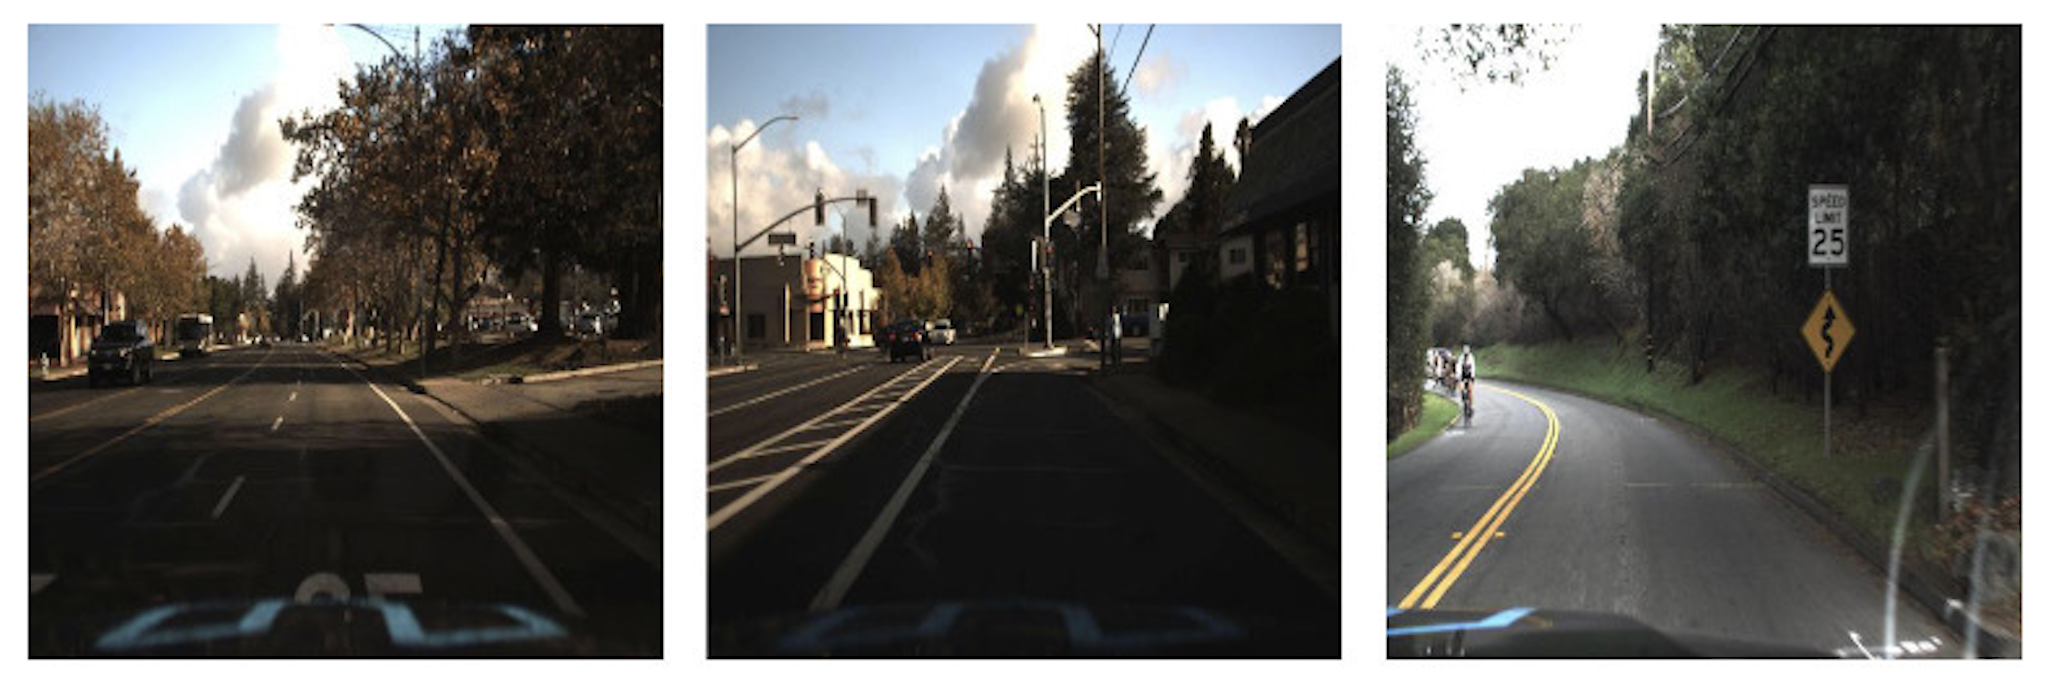
\includegraphics[width=0.55\linewidth]{datasetImages.png}
	\caption[Beispielbilder aus dem Datensatz]{Beispielbilder aus dem Datensatz. Quelle: \cite{datasetSelfDrivingCar}}
	\label{fig:datasetImages}
\end{figure}

Die Bilder in dem Datensatz umfassen verschiedene Szenarien im Straßenverkehr. Darunter befinden sich Stadt- und Landstraßen. Die Bilder wurden bei unterschiedlichen Lichtbedingungen aufgenommen, um ein breite Vielfalt an Situationen in den Daten abzudecken. 


\section{Klassenaufteilung}
Die ursprüngliche Klasseneinteilung ist in Abbildung \ref{fig:classDistributionRaw} dargestellt. Dort lässt sich erkennen, dass insbesondere die Aufteilung der Klasse \textit{Ampel} in Unterkategorien unterrepräsentiert ist. Um dieses Problem zu umgehen, wurden die \textit{Ampel}-Klassen zu einer Klasse \textit{trafficLight} zusammengeführt. Für das Auswerten des Datensatzes wurde dieser mit dem passenden Skript (datasetPreprocessing.ipynb) in einen Trainings-, Validierungs- und Testdatensatz aufgeteilt. Diese Aufteilung kann aus den farblichen Säulen in Abbildung \ref{fig:datasetTrainValTestSplit} entnommen werden. Eine weitere Bearbeitung des Datensatzes wurde nicht vorgenommen, um zu überprüfen, wie die verwendeten Netzwerke mit einem unbalancierten Datensatz umgehen. 

\begin{figure}
	\begin{subfigure}{0.5\textwidth}
		\centering
		\begin{tabular}{l|c|c}
			\hline
			Klassen & Anzahl & Index \\
			\hline
			\hline
			car & 64399 & 0 \\
			pedestrian & 10806 & 1 \\
			trafficLight-Red & 6870 & 2 \\
			trafficLight-Green & 5465 & 3 \\
			truck & 3623 & 4 \\
			trafficLight & 2568 & 5 \\
			biker & 1846 & 6 \\
			trafficLight-RedLeft & 1751 & 7 \\
			trafficLight-GreenLeft & 310 & 8 \\
			trafficLight-Yellow & 272 & 9 \\
			trafficLight-YellowLeft & 14 & 10 \\
			\hline
		\end{tabular}
		\caption{Klassenverteilung der rohen Daten als Tabelle}
		\label{tab:classDistributionRaw_graph}
	\end{subfigure}%
	\begin{subfigure}{0.5\textwidth}
	\centering
	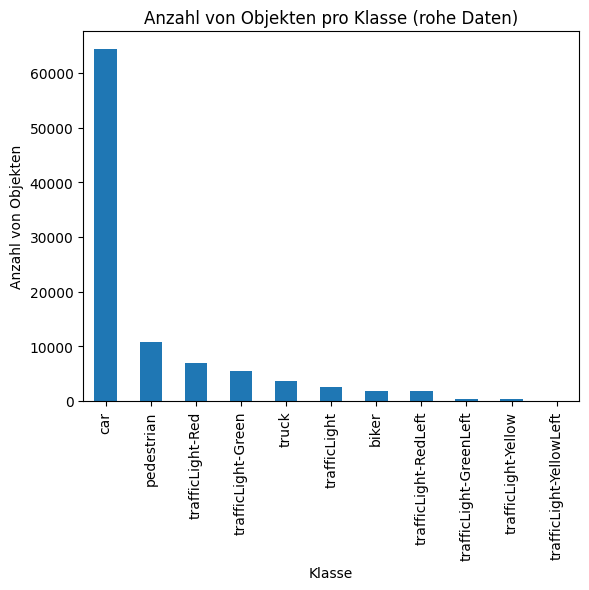
\includegraphics[width=\linewidth]{classDistribution_raw.png}
	\caption[Klassenverteilung der rohen Daten als Diagramm]{Klassenverteilung der rohen Daten als Diagramm. Quelle: Eigene Aufnahme}
	\label{fig:classDistributionRaw_graph}
	\end{subfigure}%
	\caption{Klassenverteilung der rohen Daten}
	\label{fig:classDistributionRaw}
\end{figure}


\begin{figure}
	\centering
		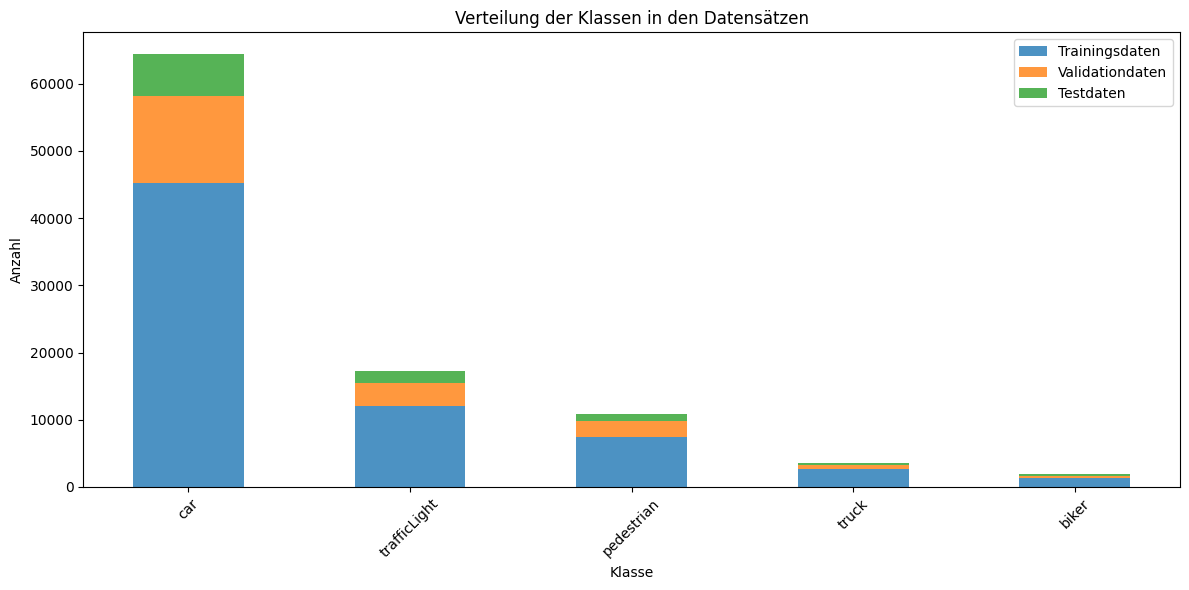
\includegraphics[width=\linewidth]{classDistribution_newClassesTrainValTest.png}
		\caption[Aufteilung in Trainings-, Validation- und Testdaten]{Aufteilung in Trainings-, Validation- und Testdaten. Quelle: Eigene Aufnahme}
		\label{fig:datasetTrainValTestSplit}
\end{figure}


\section{Aufbau}
\subsection{Rohdaten}
Die Rohdaten sind in einem Ordner gespeichert. Dieser Ordner enthält die Bilder im .jpg-Format und eine .csv-Datei in der alle Annotationen enthalten sind. Der Header der Datei enthält den Dateinamen des Bildes, die Breite und Höhe, die Klasse und die vier Bounding Box Koordinaten zu jedem Objekt.

Die folgenden Umwandlungen in die Formate werden mit dem Skript \textit{datasetConvertion.ipynb} gemacht. Die jeweiligen Ordnerstrukturen können in Kapitel \ref{chap:appendix} nachgelesen werden.


\subsection{YOLOX}
Das Netzwerk kann das COCO-Format und das PASCAL VOC-Format verarbeiten. In der folgenden Arbeit wird das COCO-Format verwendet. Zu diesem Zweck werden die Annotationen in einem separaten Ordner und die jeweiligen Bilddateien für Training, Validierung und Test ebenfalls in einem separaten Ordner abgelegt. Die Annotationen zu den drei Teildatensätzen liegen im .json-Format vor. Dabei wird jeder Klasse, jedem Bild und jeder Annotation eine ID zugewiesen, die die Zuordnung der Objekte zu den jeweiligen Bildern ermöglicht. 



\subsection{YOLOv8}
Dieses Netzwerk verwendet das YOLO-Format. Dabei werden die Bilder für Training, Validierung und Test in einem separaten Ordner gespeichert. Die dazugehörigen Labels stehen in einzelnen .txt-Dateien. Jedes Bild erhält eine zugehörige Textdatei mit dem gleichen Namen wie das Bild und der Struktur Klasse, x-Zentrum, y-Zentrum, Breite und Höhe. Die Koordinaten müssen auf die Bildgröße normiert sein. Die Labels liegen in einer korrespondierenden Ordnerstruktur. Die zugehörige Konfigurationsdatei gibt anschließend den Pfad zu den Datensatz und die Anzahl der Klassen an. 




  \chapter{Übersicht über die Modelle}
\section{YOLOX}\label{chap:yolox}
\subsection{Architektur}

\begin{figure}[h]
	\centering
	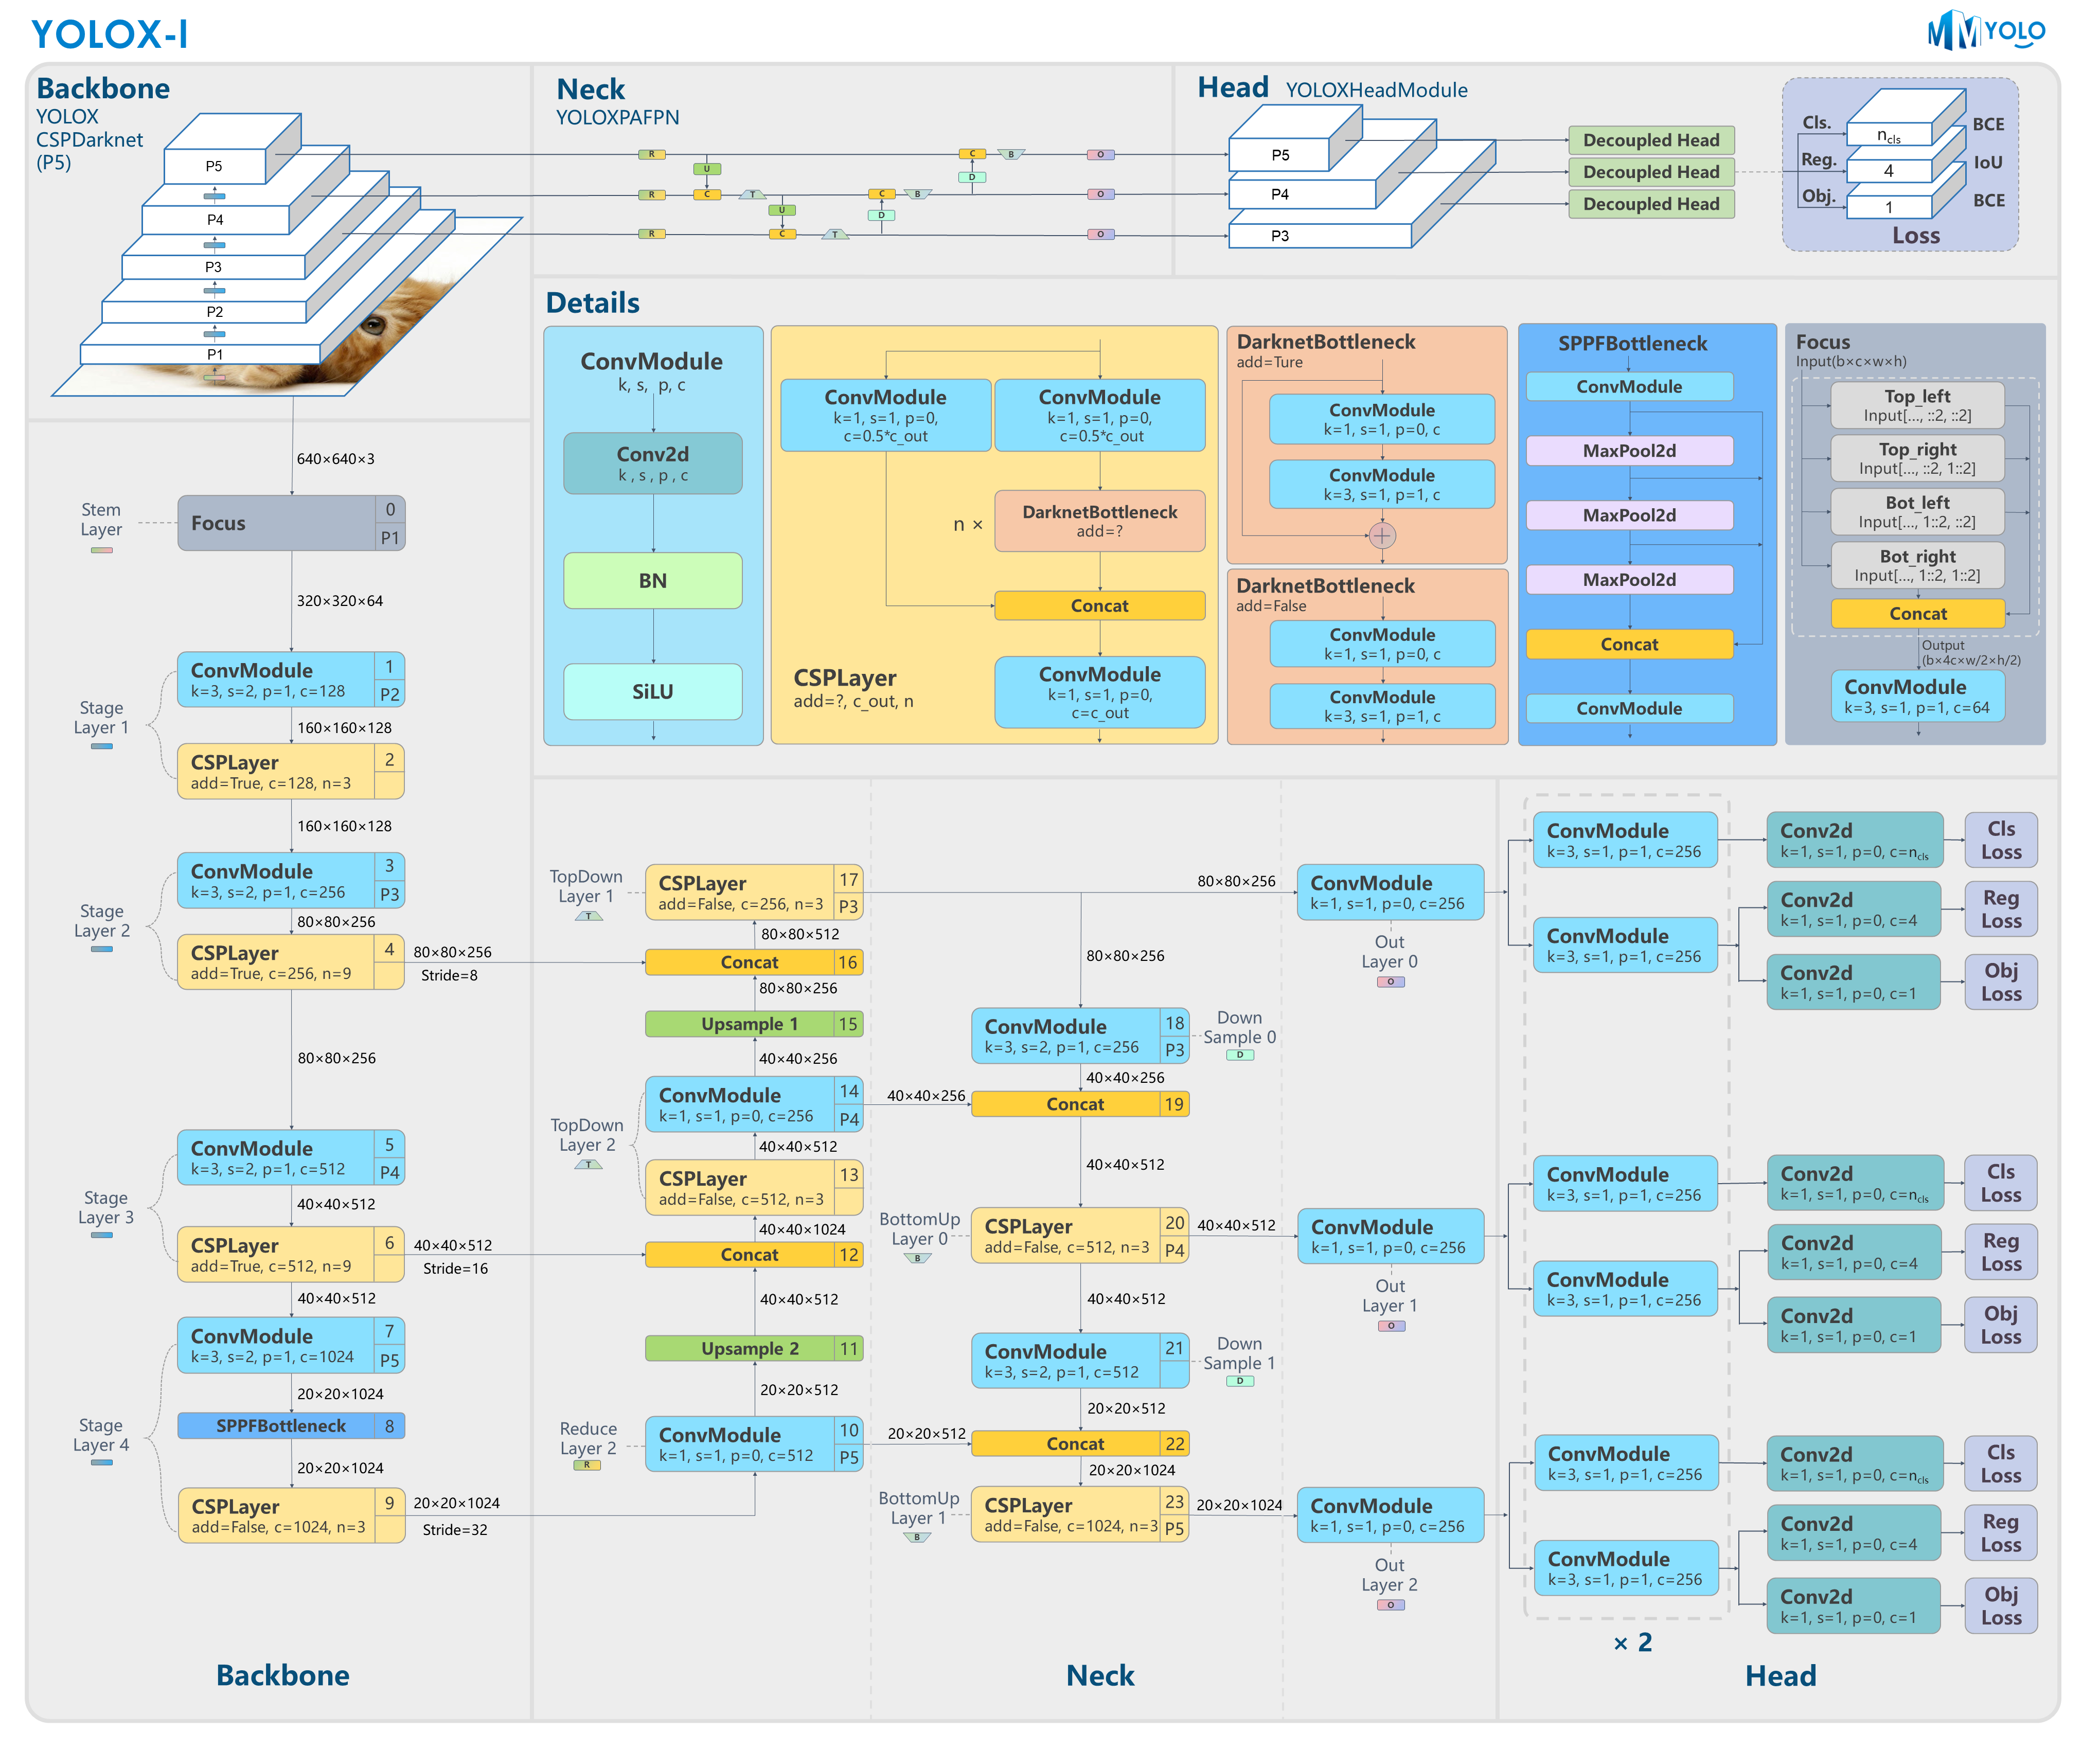
\includegraphics[width=0.8\linewidth]{yoloxArchitecture.png}
	\caption[Übersicht über die Architektur von YOLOX]{Übersicht über die Architektur von YOLOX. Quelle: \cite{yoloArchitecture, yoloxPaper, yoloxGitHubRepo}}
	\label{fig:yoloxArchitecture.png}
\end{figure}

Die YOLOX Architektur besteht aus einem Backbone-Netz, dem Neck und einem Head.

\subsubsection{Backbone}
YOLOX verwendet das CSPDarknet als Backbone, um Merkmale auf drei verschiedenen Ebenen zu extrahieren. Die Ausgänge haben Dimensionen von ($H/8$x$W/8$x$256$), ($H/16$x$W/16$x$512$) und ($H/32$x$W/32$x$1024$). Diese Skalierungen ermöglichen die Erzeugung von Merkmalen für unterschiedliche Größen von Objekten. Durch die erhöhte Anzahl von Kanälen wird der Informationsverlust in den kleineren Feature-Maps ausgeglichen. Die tiefere Feature-Map (auf der Abbildung \ref{fig:yoloxArchitecture.png} unten) besitzt ein größeres Receptive Field und ein Pixel kodiert Informationen über einen größeren Bereich des ursprünglichen Bildes.

Das CSPDarknet (Cross Stage Partial) ist eine Modifizierung des ursprünglichen Darknet-Frameworks, das in YOLOv3 schon implementiert wurde. Die Anpassungen bieten Verbesserungen in Bezug auf Geschwindigkeit und Genauigkeit bei der Erkennung von Objekten in Bildern.

CSP steht für Cross Stage Partial Network. Diese Architektur besteht aus einem CSP-Block, der in verschiedenen Stufen des Netzwerks eingefügt ist. Der CSP-Block spaltet den Eingang in zwei Zweige auf, wobei ein Teil unverändert durch den Block läuft und der andere Teil durch eine Kombination aus Faltungsoperationen und Verbindungsschichten verarbeitet wird. Das Ziel dieser Kombination ist es, eine effizientere Erfassung des Netzes auf den verschiedenen Ebenen zu ermöglichen.

In dem Backbone wird außerdem noch am Ende der Verarbeitung ein SPP verwendet. SPP steht für Spartial Pyramid Pooling. Sie ermöglicht es Objekte unterschiedlicher Größen besser zu erkennen. Dass SPP-Modul teilt das Eingangsbild auf und reduziert die Dimensionen mithilfe von mehreren Pooling Operationen. Die unterschiedlichen Stufen werden anschließend wieder miteinander verbunden und weitergereicht. Ziel dieses Moduls ist es Informationen von verschiedenen Skalierungen zu verbinden, um eine verbesserte Erkennung von Objekten zu gewährleisten. \cite{yoloxBackbone}

\subsubsection{Neck}
YOLOX verwendet im Neck das PAFPN (Path Aggregation Feature Pyramid Network). Dies ist eine Kombination des PAN (Path Aggregation Network) und dem FPN (Feature Pyramid Network). 

Das PAN ist verantwortlich für die Zusammenführung von Informationen aus verschiedenen Netzwerkpfaden und die Integration dieser Informationen in einen einzigen Satz von Merkmalen. Es verbindet die Ausgänge des Backbone-Netzwerks auf unterschiedlichen Skalierungsebenen und passt die Dimensionen durch Upsampling aneinander an. Dadurch soll das Netzwerk ein umfassenderes Verständnis, über die aus dem Backbone generierten Merkmale erhalten.

Das FPN ermöglicht eine robuste Objekterkennung in Bildern unterschiedlicher Skalierungen. Das Netzwerk erzeugt eine Hierarchie von Feature-Maps auf verschiedenen Skalierungen und verbindet sie miteinander. Dadurch sollen feine Details und auch semantische Informationen erfasst werden. FPN verwendet top-down und bottom-up-Verbindungen, um die Merkmale auf verschiedenen Ebenen des Netzwerks zu aggregieren. Die sich daraus ergebende Merkmalspyramide wird an den Head weitergeleitet. \cite{yoloxNeckPAN, yoloxNeckFPN}


\subsubsection{Head}
Der Head befindet sich am Ende des Netzwerks und ist für die Vorhersage der Objekte und deren Positionen in den Eingabebildern zuständig. Dort wird die Verlustfunktion berechnet. YOLOX verwendet einen Decoupled Head, der aus zwei Teilen besteht. Dieser Mechanismus ist mit YOLOX neu eingeführt worden und wird in Kapitel \ref{chap:decoupledHead} beschrieben.


\subsection{Methoden}
\subsubsection{Decoupled Head}\label{chap:decoupledHead}
Der Decoupled Head trennt die Vorhersage von Objekten und Bounding-Boxes in zwei Zweige auf. Zusätzlich zum Pfad der Bounding-Box wird dort der Konfidenzwert vorhergesagt. Bei den herkömmlichen YOLO-Netzwerken wird die Vorhersage (Klasse, Bounding Box und Konfidenzwert) in einer einzigen Vorhersage gemacht. Dies kann zu Schwierigkeiten bei der Erkennung von Objekten unterschiedlicher Größe führen. 

Wie in der Abbildung \ref{fig:decoupledHead} (unten) zu sehen ist, wird im Decoupled Head die Dimension des Eingangs durch eine 1x1-Faltung reduziert und anschließend in zwei Pfade aufgeteilt. Das bedeutet, dass das Modell zuerst die Präsenz von Objekten vorhersagt und in einem parallelen Zweig die Bounding-Box-Koordinaten und den Objektscore für die erkannten Objekte berechnet. Dieser Head wird für jede der drei Neck-Feature-Maps ausgeführt. \cite{yoloxExplanationHowWorks}

Die drei Tensorausgaben von YOLOX enthalten die gleichen Informationen wie die Ausgänge des großen Tensors von YOLOv3:
\begin{itemize}
\item Cls: Die Klasse jeder Bounding Box
\item Reg: Die 4 Teile der Bounding Box
\item Obj: Wie sicher ist das Netzwerk, das innerhalb der Bounding Box ein beliebiges Objekt ist
\end{itemize}


\begin{figure}[h]
	\centering
	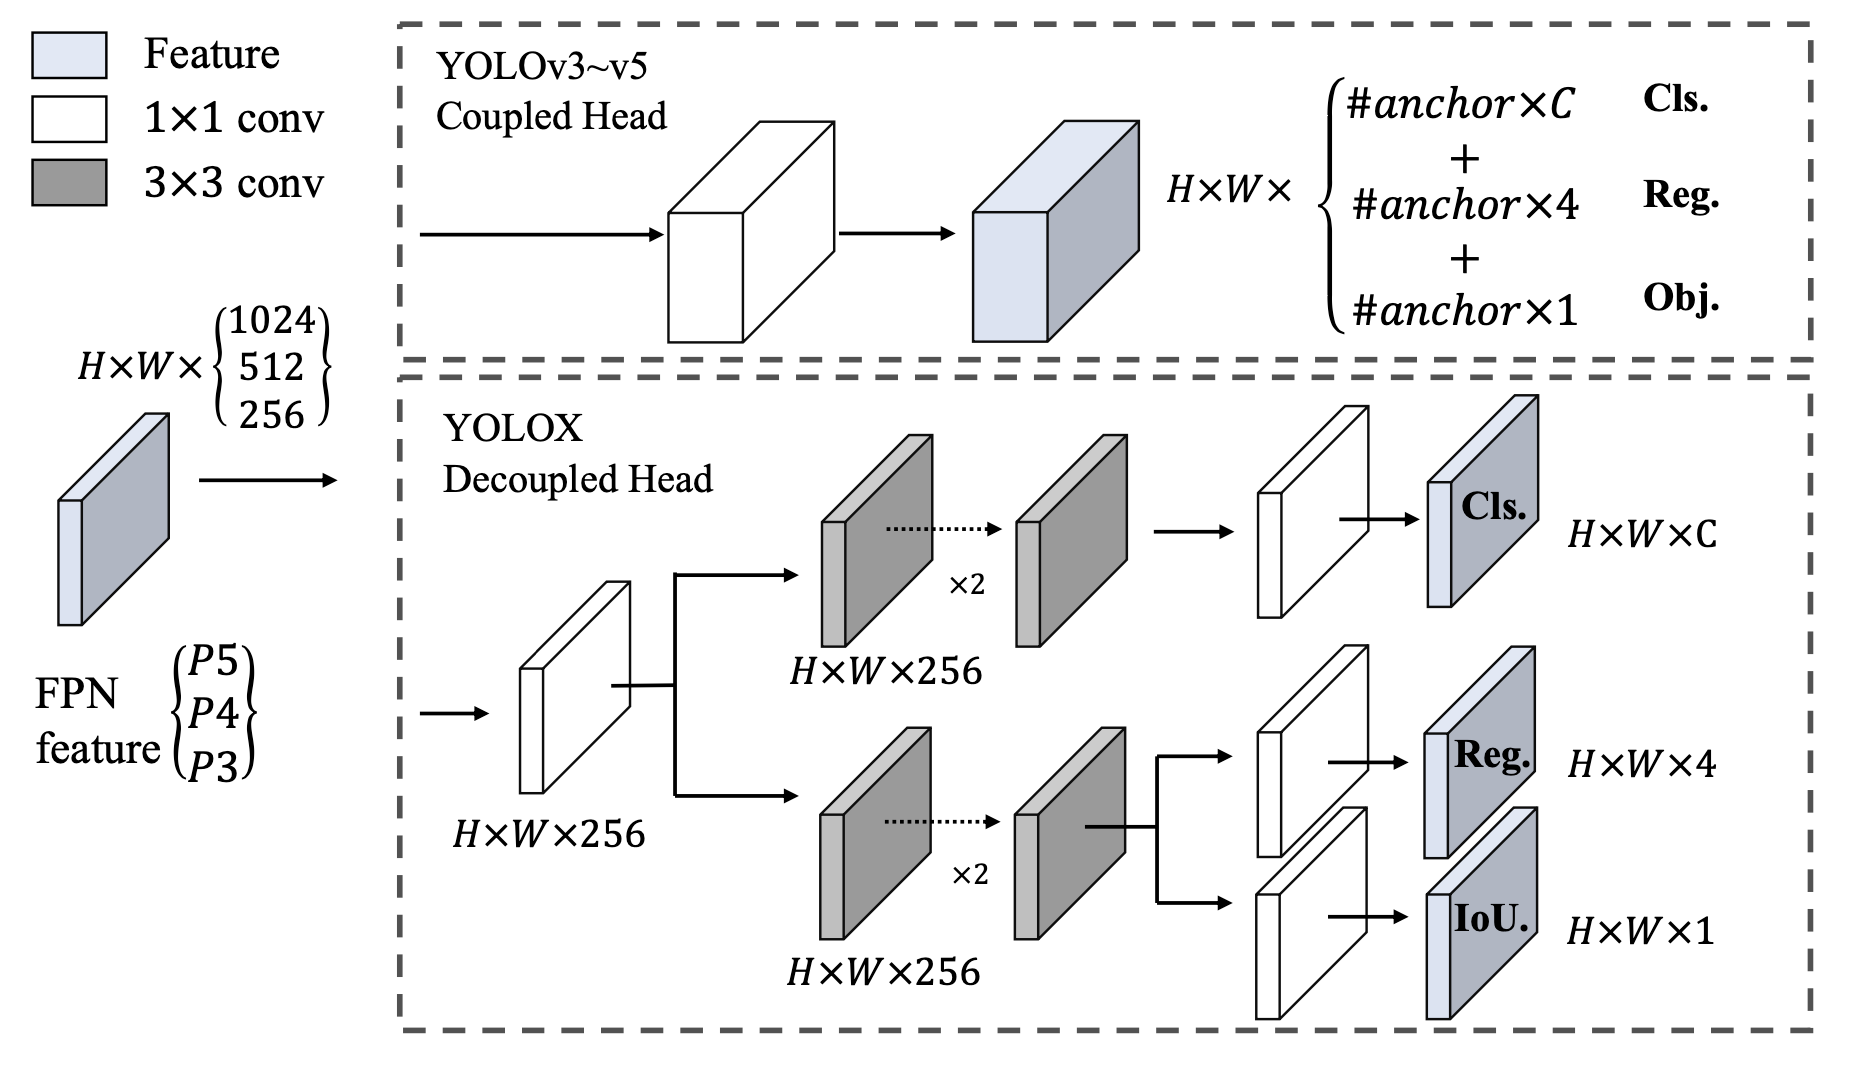
\includegraphics[width=0.55\linewidth]{decoupledHead.png}
	\caption[Illustration des Unterschieds zwischen dem Yolov3-Head und dem neuen Decoupled-Head ]{Illustration des Unterschieds zwischen dem YOLOv3-Head und dem neuen Decoupled-Head. Quelle: \cite{yoloxPaper}}
	\label{fig:decoupledHead}
\end{figure}




\subsubsection{Anchor Free Prediction}\label{chap:anchorFree}
Bei der \textbf{Anchor-based Prediction} werden vordefinierte Ankerboxen verwendet, um Objekte in verschiedenen Größen zu repräsentieren. Diese Ankerboxen dienen als Referenzpunkte, auf die die Modelle während des Trainings ausgerichtet werden. Das Modell weist der Ground-Truth (Echten) Box die ähnlichste Ankerbox zu und sagt die Verschiebung und Abmessungen der Ankerbox voraus, um sie dem Objekt anzupassen. Dazu muss vor Beginn des Trainings die Skalierung und Anzahl der Ankerboxen vorgegeben werden. Im Grunde ist eine Ankerbox eine Hilfe für das Modell, damit es nicht direkt eine Bounding Box vorhersagen muss.


Die implementierte Methode zur \textbf{Anchor-Free Predictio}n entstammt ursprünglich aus dem Paper ''FCOS: Fully Convolutional One-Stage Object Detection'' \cite{yoloxAnchorFree}. Anstelle von Ankerboxen verwendet die Anchor-Free-Methode ein Grid-basiertes Konzept. Im YOLOX Algorithmus wird eine Stride von 32, 16 und 8 verwendet, um die Ausgabebilder des Necks in ein Gitter zu unterteilen. Wenn ein Stride von 32 für ein 256×256 großes Bild verwendet wird, ergeben sich insgesamt 256/32 = 8 Schnittpunkte in jeder Dimension, also insgesamt 64 Schnittpunkte. Jeder dieser Schnittpunkte heißt Ankerpunkt. Ein Ankerpunkt ist ein Offset, mit dem die (x, y)-Position einer Vorhersage verschoben wird. Die Position des Ankers kann auf dem Bild mit den folgenden Formeln ermittelt werden:
\begin{align}
	x = \frac{s}{2} + s*i, \qquad y = \frac{s}{2} + s*j
\end{align}
Dabei ist \textit{s} die Schrittweite, \textit{i} ist der i-te Schnittpunkt auf der x-Achse und \textit{j} ist der j-te Schnittpunkt auf der y-Achse. Bei YOLOX werden die Gitterpunkte als linker oberer Offset der Bounding Box verwendet. Die folgenden Formeln werden verwendet, um eine vorhergesagte Bounding Box $(p_x, p_y, p_w, p_h)$ auf die tatsächliche Position auf dem Bild $(l_x, l_y, l_w, l_h)$ abzubilden, wenn (x, y) der Schnittpunkt auf dem Gitter ist, zudem die Vorhersage gehört und s die Schrittweite der aktuellen FPN-Ebene ist:
\begin{align}
	l_x=p_x+x, \qquad l_y=p_y+y, \qquad l_w=s*e^{p_w}, \qquad l_h=s*e^{p_h}
\end{align}
Wir verschieben den vorhergesagten Punkt, indem wir die Vorhersage zum Anker-Punkt (dem (x,y)-Punkt, der dieser Vorhersage zugewiesen ist) hinzufügen. Durch die e-Funktion wird sichergestellt, dass die Höhe und Breite nicht negativ ist und verschieben diese auf der Grundlage der Schrittweite s eines Bildes. Das Beispiel zu dieser Methode kann in der angegeben Quelle nachgelesen werden. \cite{yoloxExplanationHowWorks}


\subsubsection{SimOTA Label Assignment}\label{chap:simota}
Die Methode soll die Zuordnung der Vorhersagen zu den Ground-Truth-Objekten optimieren, da nicht alle Vorhersagen gut sind und das Modell nicht versuchen soll diese zu optimieren. Dazu werden die Ankerpunkte der vorherigen Methode von \ref{chap:anchorFree} in positive und negative Gruppen aufgeteilt.

OTA (Optimal Transport Assignment) ist ein Ansatz, der das Zuordnungsproblem in der Objekterkennung als Optimal Transport (OT)-Problem formuliert. Es geht darum, den besten Plan zu finden, um Güter (Objekte) von Anbietern (Ground-Truth) zu Nachfragern (Vorhersagen oder Anker) zu minimalen Kosten zu transportieren. OTA verwendet OT, um die Labels den Ankerorten zuzuweisen und die Anker als positiv oder negativ zu kennzeichnen. Der Hintergrund wird als zusätzlicher \glqq Lieferant\grqq\ betrachtet. 

Das Problem des OTA-Algorithmus ist, dass dieser das Training verlangsamt. Aus diesem Grund gibt es eine Vereinfachung des Algorithmus, indem der optimale Zuweisungsplan angenähert wird. Vereinfacht funktioniert der Algorithmus folgendermaßen:
\begin{itemize}
	\item Berechne die Klassen- und Regressionsvorhersage für eine gegebene Eingabe durch das Modell.
	\item Erstelle einen Liefervektor, der das Angebot (durch Dynamic k estimation festgelegt) für jeden der Ground-Truths repräsentiert.
	\item Initialisiere den Nachfragevektor mit Einsen für jede Vorhersage.
	\item Berechne die Kosten für Klassenverluste ($FocalLoss(P^{cls}, G^{cls})$), Regressionsverluste ($IoULoss(P^{cls}, G^{cls})$))) und Zentrumsprior zwischen Vorhersagen und Ground-Truths.
	\item Berechne die Kosten für den Hintergrund und den Vordergrund basierend auf den Kosten der einzelnen Komponenten.
	\item Konstruiere eine Kostenmatrix, die die Hintergrund- und Vordergrundkosten enthält.
	\item Wähle die besten Vorhersagen basierend auf den Kosten und dem verfügbaren Angebot.
	\item Gebe die ausgewählten Vorhersagen zurück.
\end{itemize}

Der SimOTA-Algorithmus verwendet das Konzept von Angebot und Nachfrage, um die optimale Zuordnung zwischen Vorhersagen und Ground-Truths zu finden. Durch die Berücksichtigung von Kosten und verfügbaren Angebot werden die besten Vorhersagen ausgewählt, um eine präzisere Objekterkennung zu ermöglichen. Der vollständige Algorithmus kann in der angegeben Quelle nachgelesen werden.  \cite{yoloxExplanationSimOTA}


\subsubsection{Advanced Augmentation}\label{chap:advancedAug}
YOLOX verwendet Advanced Data Augmentation-Techniken wie Mosaic und MixUp, um die Datenvielfalt während des Trainings zu erhöhen und die Leistungsfähigkeit des Modells zu verbessern.

Beim \textbf{Mosaic}-Verfahren werden vier zufällig ausgewählte Bilder aus dem Trainingsdatensatz genommen und zu einem Mosaikbild kombiniert. Dabei werden die Bilder in vier quadratische Bereiche aufgeteilt und zu einem einzigen großen Bild zusammengefügt. Die Bounding Boxes der Objekte werden entsprechend angepasst und die Klassenlabels beibehalten. Mithilfe des CutOuts wird ein beliebiger Teil aus dem Bild ausgeschnitten und die Bounding Boxen noch einmal angepasst. Das Mosaikbild wird dann als Eingabe für das Modell verwendet. Der Grund für die Verwendung von Mosaic ist, dass es die Fähigkeit des Modells verbessert, mit komplexen Szenarien und Objektüberlappungen umzugehen.

\textbf{MixUp} ist eine Technik, bei der zwei zufällig ausgewählte Bilder und ihre entsprechenden Bounding Boxen und Klassenlabel gemischt werden, indem ihre Annotationen gewichtet kombiniert werden. Das erste Bild wird mit $\lambda$ und das zweite Bild mit $1-\lambda$ multipliziert. Die beiden resultierenden Ergebnisse werden addiert. \cite{yoloxExplanationAug}

\begin{figure}[h]
	\centering
	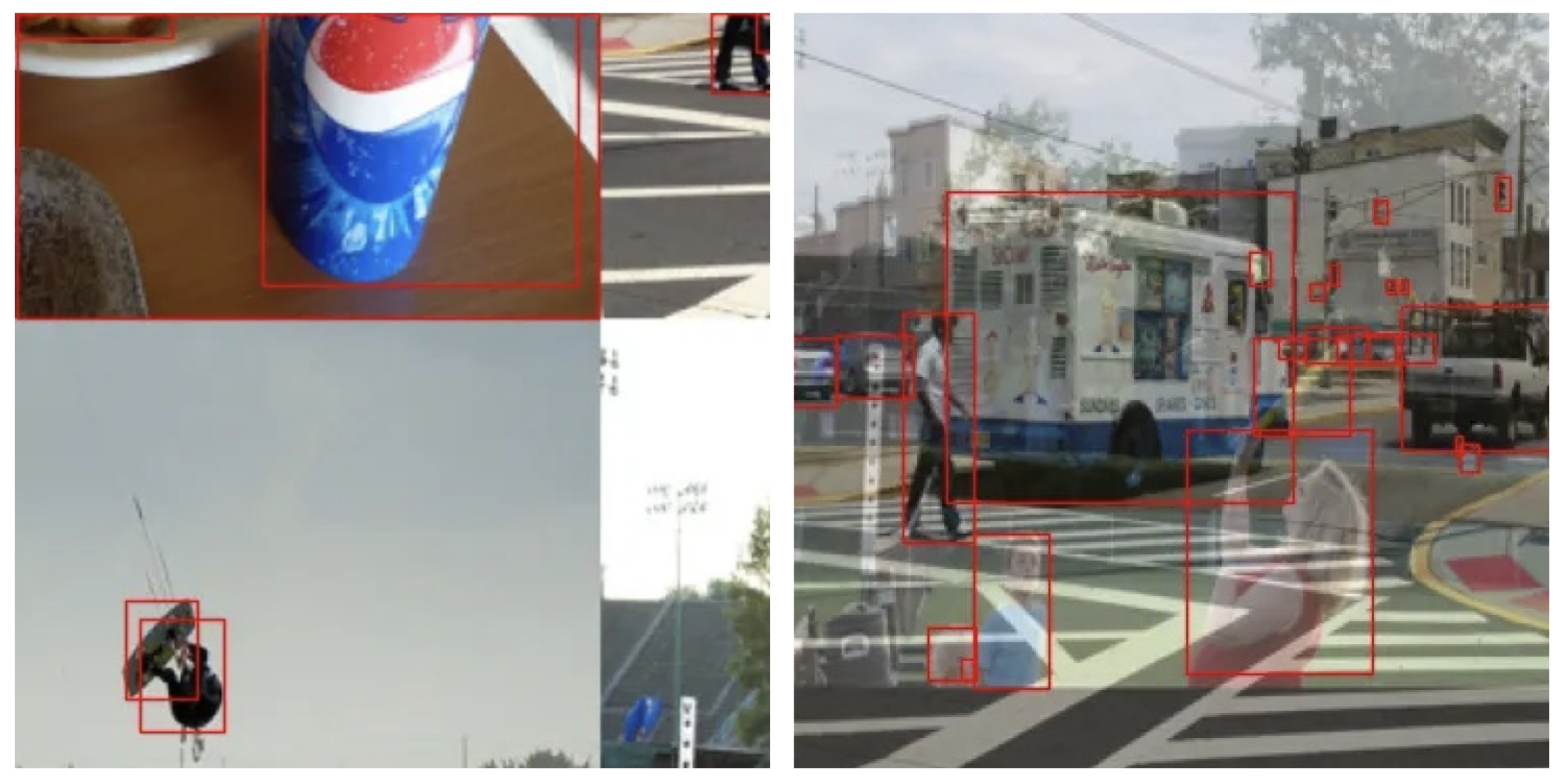
\includegraphics[width=0.55\linewidth]{dataAugmentation.png}
	\caption[Beispielbild nach Anwendung der beiden Data Augmentation Methoden]{Beispielbild nach Anwendung der beiden Data Augmentation Methoden (links: Mosaic, rechts: MixUp) Quelle: \cite{yoloxExplanationAug}}
	\label{fig:yoloxExplanationAug}
\end{figure}



\subsection{Verlustfunktion}
\subsubsection{Gesamtverlust}
Die Gesamtverlustfunktion des Modells setzt sich aus drei einzelnen Verlustfunktionen für die jeweiligen Aufgaben zusammen:

\begin{align}
	\mathcal{L}^{total}=\frac{1}{N_{pos}}*\mathcal{L}^{cls}+\alpha*\frac{1}{N_{pos}}*	\mathcal{L}^{iou}+	\frac{1}{N_{pos}}*\mathcal{L}^{obj}
\end{align}

Die Verlustfunktion ist dabei die Summe der einzelnen Komponenten, gemittelt über die Menge der positiven Labels. Die positiven Labels werden durch SimOTA (\ref{chap:simota}) bestimmt. Der Parameter $\alpha$ ist ein Gewichtungsterm, der von den Autoren des Papers auf $5.0$ festgelegt ist.

\subsubsection{Klassifikation}\label{chap:yoloxClassification}
Für die Verlustfunktion des Klassifikationsteils, verwendet YOLOX die Binary Cross Entropy (BCE) mit Logits. Dabei handelt es sich um die normale BCE-Funktion mit einer vorgeschalteten Sigmoidfunktion für die Prognosen.

Die Formel lautet:
\begin{align}
	\mathcal{L}^{cls}=\frac{1}{N}\sum_{i}^{N}y_i*log(\sigma(\hat{y_i}))+(1-y_i)*log(1-\sigma(\hat{y}_i))\text{,}
\end{align}

wobei $\hat{y}$ der Vektor der Klassenvorhersagen für C Klassen ist. Die Sigmoidfunktion $\sigma$ wird verwendet, um die Elemente in einem Wertebereich von [0,1] abzubilden. Die Werte in y sind ein One-Hot-Vektor, der eine 1 für die richtige Klasse und eine 0 für alle anderen Klassen enthält. Die Werte der Vektoren y und $\hat{y}$ stammen aus der positiv gekennzeichneten Menge. Das Ziel des BCE-Verlustes ist, dass das Modell lernt, eine 1 für die richtige Klasse und eine 0 für alle anderen Klassen in der Bounding Box vorherzusagen. \cite{yoloxExplanationHowWorks}

\subsubsection{Bounding Box}
In YOLOX wird die IoU (Intersection over Union) Loss Funktion verwendet, um die Regressionsverluste für die Bounding Box Koordinaten zu berechnen. Diese Loss Funktion misst die Ähnlichkeit zwischen der vorhergesagten Bounding Box und der Ground Truth Bounding Box anhand des IoU-Werts.

Der IoU-Wert wird berechnet, indem der Flächenanteil des überlappenden Bereichs der Bounding Boxen durch die Summe der Flächen beider Bounding Boxen geteilt wird. Mathematisch kann der IoU-Wert wie folgt ausgedrückt werden:

\begin{align}
	IoU = \frac{Area_{Intersection}}{Area_{Union}}\text{,} \qquad IoU \in [0,1]
\end{align}

Je höher der IoU-Wert, desto besser ist die Übereinstimmung zwischen der Vorhersage und der Ground Truth Bounding Box.

Die resultierende Verlustfunktion ist folgendermaßen definiert:
\begin{align}
	\mathcal{L}^{iou} = \frac{1}{N}\sum_{i}^{N}(1-IoU_i)^2 \text{,}
\end{align}

wobei N die Anzahl der positiven Elemente ist und die Bounding Boxen aus dieser Menge entstammen. \cite{yoloxExplanationHowWorks}

\subsubsection{Objectness}
Das Ziel des Objectness Loss in YOLOX ist es, dass das Modell einen Wert nahe 1 hat, wenn es schätzt, dass sich ein Objekt in der Bounding Box befindet, einen Wert nahe 0, wenn es schätzt, dass sich nichts in der Box befindet, und einen Wert dazwischen (vorzugsweise etwa 0.5), wenn es unsicher ist.

Um den Wert zu optimieren wird die Binary Cross Entropy with Logits verwendet, die Funktion die auch in \ref{chap:yoloxClassification} verwendet wird. Dabei werden die positiven und negativen Labels von SimOTA verwendet.

Für die positiven Vorhersagen wird der IoU-Wert zwischen vorhergesagter und Ground Truth Bounding Box verwendet, um den Wert zu bestimmen, den das Modell vorhersagen soll. Bei negativen Vorhersagen wird der größte IoU-Wert zwischen der vorhergesagten negativen Bounding Box und allen Ground Truth Bounding Boxen verwendet, um die Ground Truth Werte für die negativen Vorhersagen zu bestimmen. \cite{yoloxExplanationHowWorks}


\section{YOLOv8}\label{chap:yolov8}
\subsection{Architektur}
\begin{figure}[h]
	\centering
	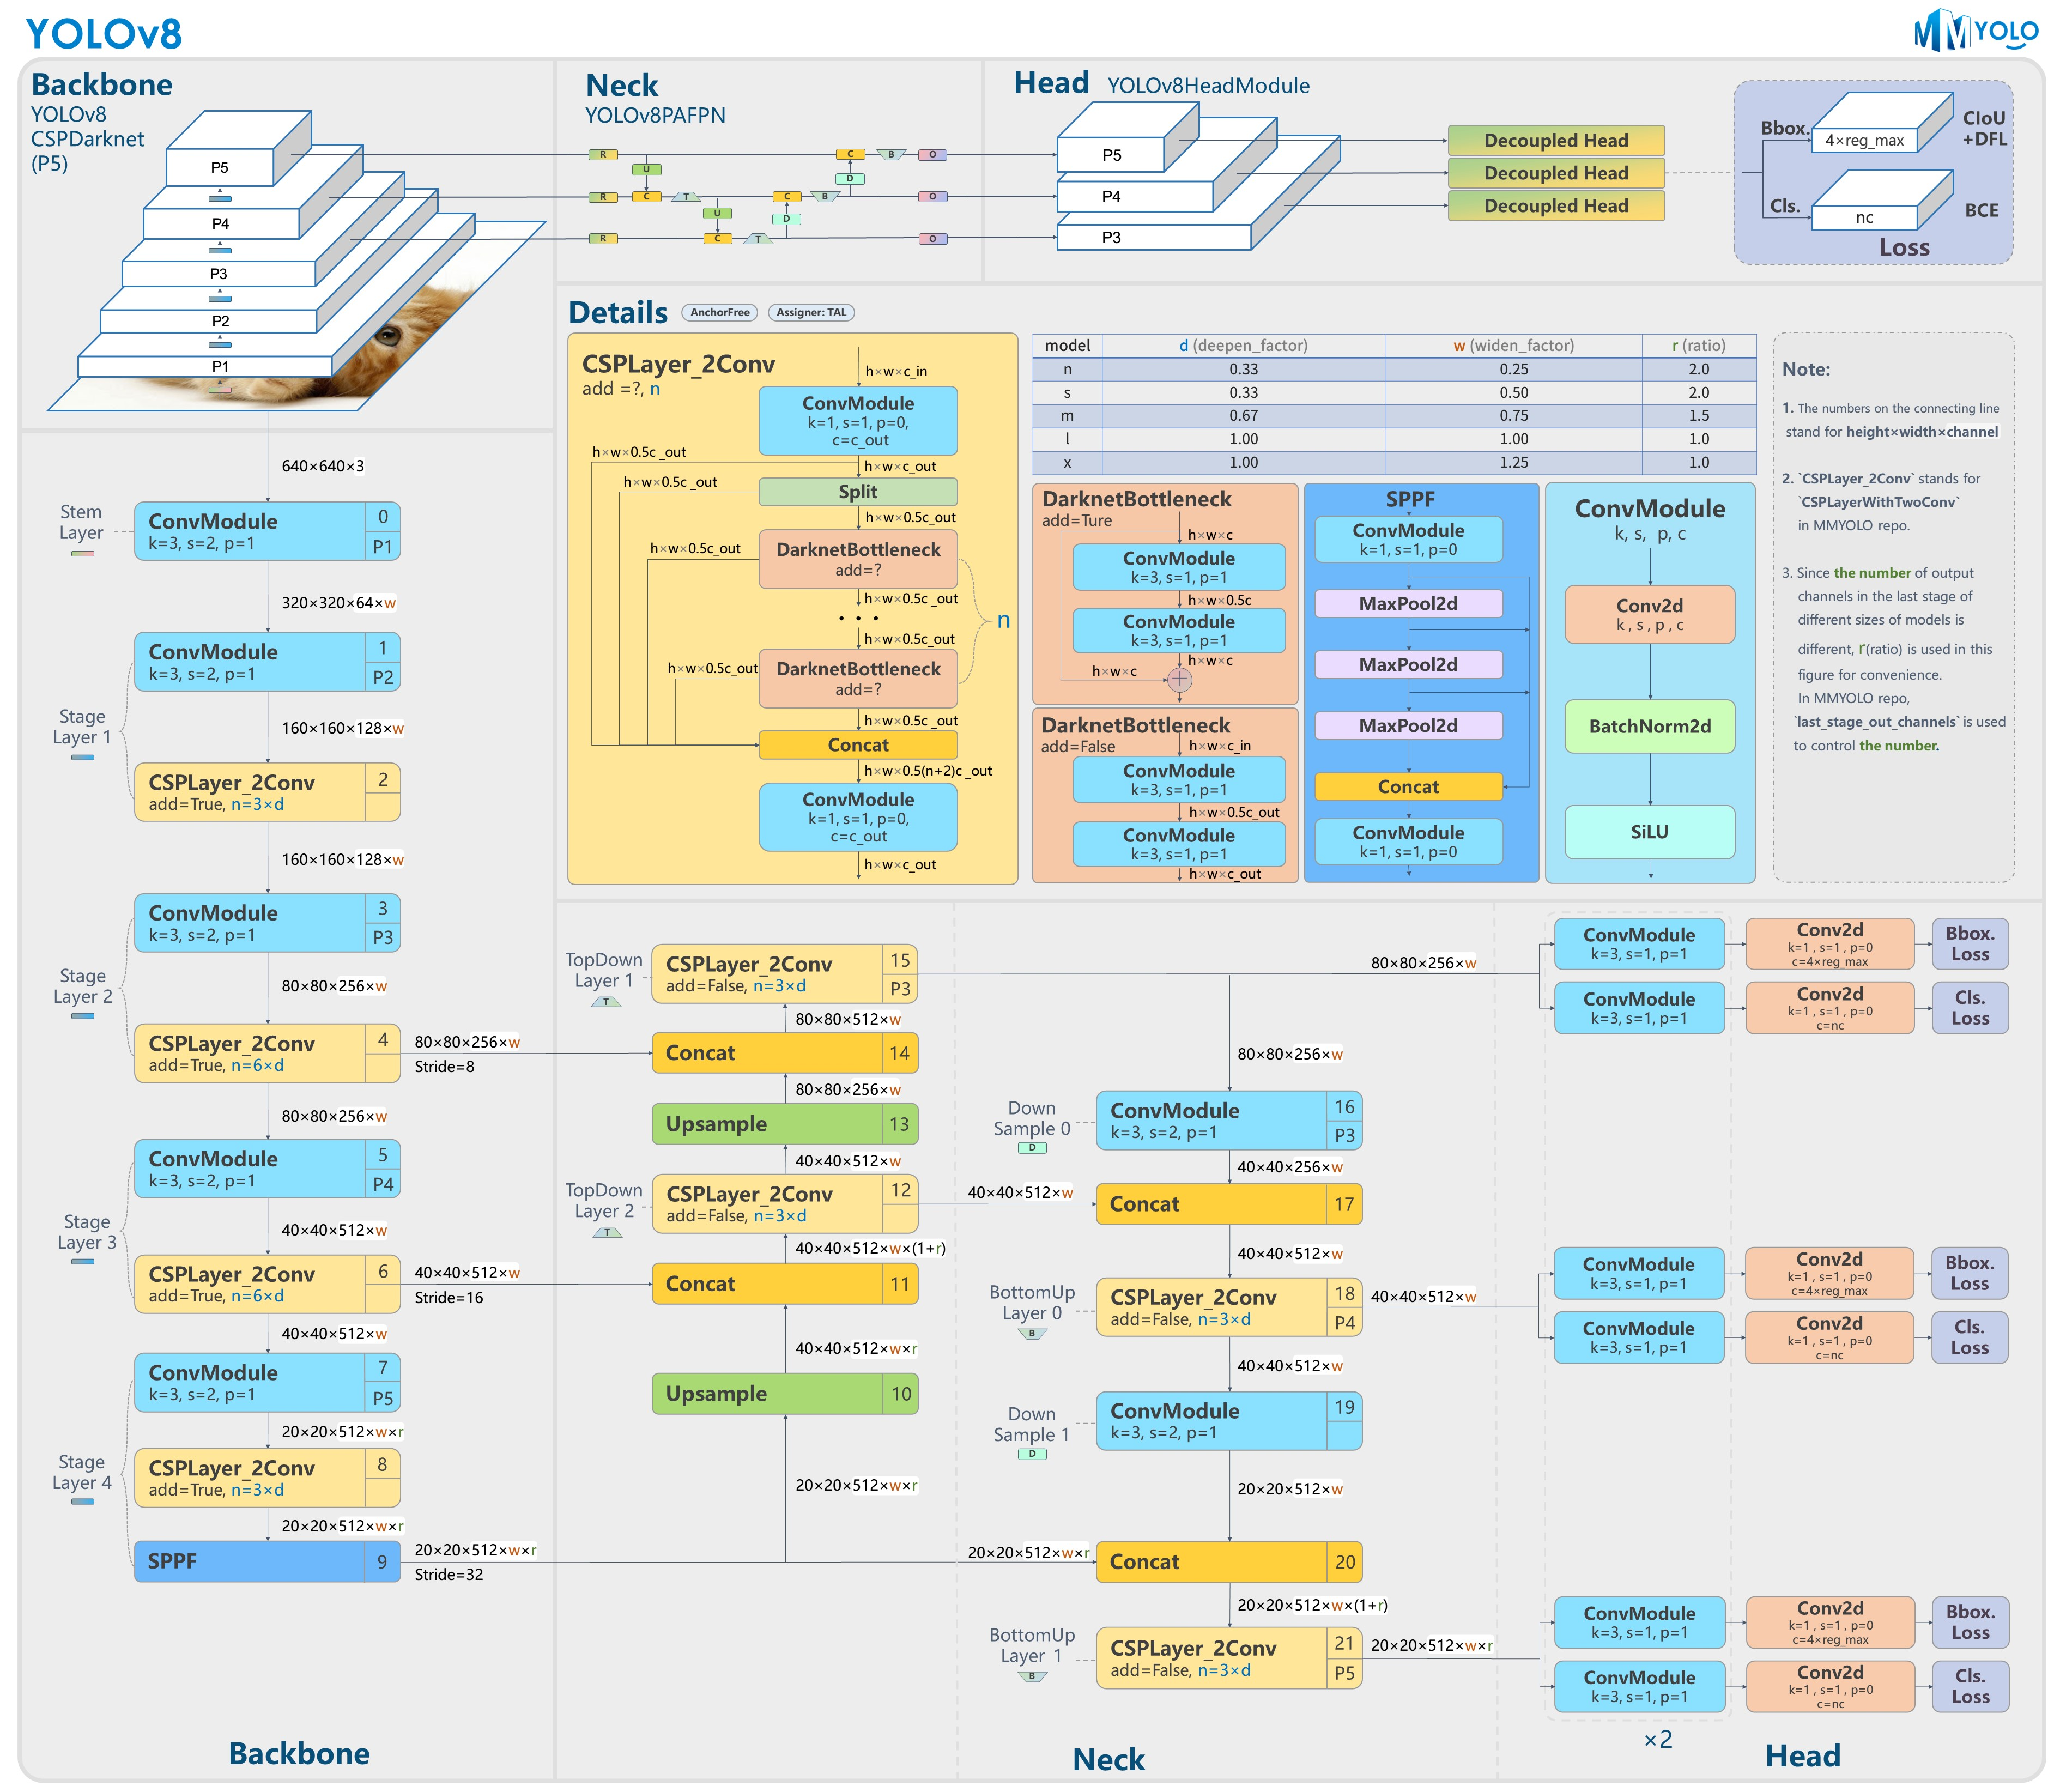
\includegraphics[width=0.8\linewidth]{yolov8Architecture.jpeg}
	\caption[Übersicht über die Architektur von YOLOv8]{Übersicht über die Architektur von YOLOv8. Quelle: \cite{yoloArchitecture}}
	\label{fig:yolov8Architecture}
\end{figure}

YOLOv8 basiert ebenfalls auf dem CSPDarknet als \textbf{Backbone}-Netzwerk, das auch von YOLOX verwendet wird. Allerdings gibt es einige Unterschiede in der Architektur. Das CSP-Modul besitzt mehr Skip-Connections, das SPP-Bottleneck-Modul ist mit einem CSP-Modul vertauscht worden und das ConvModule am Ende des Backbones wurde entfernt. Im \textbf{Neck}-Bereich des Netzwerks wurden minimale Änderungen an einzelnen Schichten vorgenommen, wie beispielsweise das Vertauschen der Position einiger ConvModule. Genaueres ist aus der Abbildung \ref{fig:yolov8Architecture} zu entnehmen.
Der \textbf{Head} des Netzwerks verwendet auch den Decoupled Head mit einer Anchor-Free-Prediction. Innerhalb des Zweigs für die Bounding Box Regression wurde die Verlustfunktion für den Objectness Score entfernt. Ähnlich wie YOLOX verwendet auch YOLOv8 während des Trainings die Mosaic-Augmentierung und die MixUp-Augmentierung. Diese Techniken dienen dazu, die Trainingsdaten zu erweitern und die Robustheit des Modells zu verbessern. \cite{yolov8ModelExplanation}

Für die Funktion des Decoupled Head mit der Anchor-Free-Prediction wird auf Seite \pageref{chap:decoupledHead} und Seite \pageref{chap:anchorFree} verwiesen. Die Datenvorverarbeitung ist unter Kapitel \ref{chap:advancedAug} beschrieben. 

\subsection{Methoden}
\subsubsection{TOOD}
Der YOLOv8-Algorithmus übernimmt die Zuweisungsstrategie von TaskAlignedAssigner, da sie als effektiv angesehen wird. Die TaskAlignedAssigner-Strategie wählt positive Proben, basierend auf gewichteten Klassifizierungs- und Regressionsergebnissen, aus. 

Die TaskAlignedAssigner verwendet eine Zuweisungsstrategie, bei der für jede Ground-Truth-Bounding Box ein Ausrichtungsmetrik-Wert für jeden Anker berechnet wird. Dieser Wert wird durch das gewichtete Produkt zweier Werte ermittelt: der vorhergesagten Klassifikationspunktzahl der entsprechenden Klasse und dem Intersection over Union (IoU) zwischen der vorhergesagten Bounding Box und der Ground-Truth-Bounding Box. Anschließend werden für jede Ground-Truth-Bounding Box die größten Top-k-Proben basierend auf den Werten der Ausrichtungsmetriken, direkt als positive Proben ausgewählt. \cite{yolov8ModelExplanation, yolov8LabelAssignment}

\subsection{Verlustfunktion}
\subsubsection{Gesamtverlust}
YOLOv8 verwendet im Klassifikationszweig das BCELoss und im Regressionszweig eine Kombination aus dem Distribution Focal Loss und dem CIoU Loss. Die drei Teilfunktionen werden anschließend gewichtet summiert:

\begin{align}
	\mathcal{L}^{total}=\lambda_{cls}*\mathcal{L}^{cls}+\lambda_{iou}\mathcal{L}^{ciou}+	\lambda_{dfl}*\mathcal{L}^{dfl} \text{,}
\end{align}

wobei $\lambda_{cls}$ auf 7.5, $\lambda_{iou}$ auf 0.5 und $\lambda_{dfl}$ auf 1.5 gesetzt ist.

\subsubsection{Klassifikation} 
Für die Verlustfunktion der Klassifikation verwendet YOLOv8 die Binary Cross Entropy (BCE) mit Logits. Dabei handelt es sich, um die BCE-Funktion mit einer vorgeschalteten Sigmoidfunktion für die Prognosen.
Die Formel lautet wie auch bei YOLOX:
\begin{align}
	\mathcal{L}^{cls}=\frac{1}{N}\sum_{i}^{N}y_i*log(\sigma(\hat{y_i}))+(1-y_i)*log(1-\sigma(\hat{y}_i)) \text{,}
\end{align}

Die Parameter können in Kapitel \ref{chap:yoloxClassification} nachgelesen werden. Die positiven Lables werden allerdings nicht durch SimOTA, sondern durch TOOD berechnet.

\subsubsection{Regression} 
Die Verlustfunktion für den Regressionzweig besteht aus zwei Teilen. Der erste Teil ist das Complete-IoU-Loss (CIoU). Der CIoU-Verlust führt im Vergleich zum IoU-Verlust zwei neue Konzepte ein:
\begin{itemize}
\item Konzept des Mittelpunktabstandes, das den Abstand zwischen dem tatsächlichen Mittelpunkt der Bounding Box und der vorhergesagten Bounding Box berechnet.
\item Konzept des Seitenverhältnisses, indem es die Seitenverhältnisse der tatsächlichen Box, mit den Seitenverhältnissen der vorhergesagten Boxen vergleicht.
\end{itemize}

Die Formel lautet:
\begin{align}
	\mathcal{L}^{iou}=\sum_{i}^{N}(1-CIoU)*weight, \qquad 	CIoU = IoU - \frac{d^2}{c^2}+\alpha*v
\end{align}
\begin{align}
	v=\frac{4}{\pi}(\arctan(\frac{w^{gt}}{h^{gt}})-\arctan(\frac{w^{dt}}{h^{dt}})), \qquad \alpha=\frac{v}{(1-IoU)+v}
\end{align}

Dabei ist $d^2$ die euklidische Distanz zwischen den Mittelpunkten der Bounding Boxen der Ground Truth (gt) und Vorhersage (dt). Der Parameter $c^2$ ist die Diagonale der kleinsten Box, die beide Bounding Boxen umschließt. Der Parameter $v$ entsteht aus den Seitenverhältnissen der Bounding Boxen und $\alpha$ ist ein Gewichtungsparameter, der eine Funktion des IoUs ist. \cite{ciouLoss}

Der zweite Teil des Regressionszweigs ist das Distributed Focal Loss. Die Formel für das DFL lautet:
\begin{align}
	\mathcal{L}^{dfl}=\frac{1}{N}\sum_{i}^{N}(CE(predDist_i, tl_i)*wl_i+CE(predDist_i, tr_i)*wr_i)
\end{align}

Das DFL verwendet eine Verteilung der Bounding Boxen, um die Vorhersage genauer anzupassen. Anstatt nur eine Box zu erzeugen, wird eine Verteilung von möglichen Bounding Boxen berücksichtigt. Die Verteilung wird durch die Ankerpunkte und einen maximalen Regressionswert definiert. Der Regressionwert legt fest, in welchen Bereich die Boxen liegen sollen. Anschließend wird die Cross-Entropy-Funktion (CE) mit dem linken Bereich der Zielverteilung und mit dem rechten Bereich der Zielverteilung berechnet. Die Ergebnisse werden mit den für die Seiten spezifischen Gewichten multipliziert. Eine detaillierte Beschreibung der Verlustfunktion kann im Paper nachgelesen werden. \cite{dflLoss}


  \chapter{Modellauswertung}
\section{Metriken}
Der mAP (mean Average Precision) ist eine Metrik zur Bewertung der Leistung von Objekterkennungsmodellen. Der mAP-Wert wird für verschiedene IoU-Schwellenwerte berechnet. mAP@0.5:0.95 deckt einen großen Bereich von IoU-Schwellen ab. Der mAP@0.5 gibt an, wie gut das Modell Objekte bei einer IoU-Schwelle von 0,5 erkennt. mAP@0.75 gibt die Leistung bei einer höheren IoU-Schwelle von 0,75 an. Diese Metriken bewerten die Erkennungs- und Lokalisierungsgenauigkeit des Modells bei verschiedenen Überlappungsschwellen (IoU-Werten). Sie dienen dem Vergleich und der Bewertung der Modelle. Ein höherer mAP-Wert bedeutet eine bessere Leistung bei der Erkennung von Objekten mit dieser spezifischen Überlappungsschwelle.

Die beiden Tabellen \ref{tab:metricVal} und \ref{tab:metricTest} liefern eine Bewertung der Leistung von YOLOX und YOLOv8 anhand verschiedener Metriken. Die erste Tabelle basiert auf dem Validierungsdatensatz, der während des Trainings zur Validierung verwendet wurde, während die zweite Tabelle den unabhängigen Testdatensatz zeigt, der zu Beginn der Arbeit abgespalten wurde.

Bei dem Vergleich der Gesamtleistung des Modells (Klasse: all) ist YOLOv8 in allen Werten um 2 \% besser als YOLOX. Die ähnlichen mAP-Werte Im direkten Vergleich der einzelnen Klassen besitzt YOLOv8 ebenfalls einen höheren mAP-Wert. Die relativ ähnlichen Werte lassen sich vermutlich auf die ähnlichen Architekturen der beiden Modelle zurückführen.

\begin{table}[!ht]
	\centering
	\renewcommand{\arraystretch}{1.1} % Anpassung der Zellhöhe
	\begin{tabular}{|l|>{\arraybackslash}p{1.5cm}|>{\arraybackslash}p{1.5cm}|>{\arraybackslash}p{1.5cm}|>{\arraybackslash}p{1.5cm}|>{\arraybackslash}p{1.5cm}|>{\arraybackslash}p{1.5cm}|}
		\hline
		\textbf{} & \multicolumn{2}{c|}{\textbf{mAP@0.5:0.95}} & \multicolumn{2}{c|}{\textbf{mAP@0.5}} & \multicolumn{2}{c|}{\textbf{mAP@0.75}} \\ \cline{2-7}
		\textbf{} & YOLOX & YOLOv8 & YOLOX & YOLOv8 & YOLOX & YOLOv8 \\ \hline
		\textbf{all} & 0.484 & \textbf{0.501} & 0.776 & \textbf{0.793} & 0.508  & \textbf{0.528} \\ \hline
		\textbf{car} & 0.567 & \textbf{0.607} & 0.845 &\textbf{ 0.873} & 0.633 & \textbf{0.684} \\ 
		\textbf{pedestrian} & \textbf{0.348} & 0.342 & \textbf{0.690} & 0.67 & \textbf{0.307} & 0.297 \\
		\textbf{trafficLight} & 0.473 & \textbf{0.499} & 0.784 & \textbf{0.831} & 0.465 & \textbf{0.501} \\
		\textbf{truck} & 0.628 & \textbf{0.646} & 0.864 & \textbf{0.877} & 0.726 & \textbf{0.743} \\
		\textbf{biker} & 0.403 & \textbf{0.412} & 0.696 & \textbf{0.713} & 0.412 & \textbf{0.416} \\ \hline
	\end{tabular}
	\caption{Vergleich der mAP Werte für den Validierungsdatensatz}
	\label{tab:metricVal}
\end{table}

\begin{table}[!ht]
	\centering
	\renewcommand{\arraystretch}{1.1} % Anpassung der Zellhöhe
	\begin{tabular}{|l|>{\arraybackslash}p{1.5cm}|>{\arraybackslash}p{1.5cm}|>{\arraybackslash}p{1.5cm}|>{\arraybackslash}p{1.5cm}|>{\arraybackslash}p{1.5cm}|>{\arraybackslash}p{1.5cm}|}
		\hline
		\textbf{} & \multicolumn{2}{c|}{\textbf{mAP@0.5:0.95}} & \multicolumn{2}{c|}{\textbf{mAP@0.5}} & \multicolumn{2}{c|}{\textbf{mAP@0.75}} \\ \cline{2-7}
		\textbf{} & YOLOX & YOLOv8 & YOLOX & YOLOv8 & YOLOX & YOLOv8 \\ \hline
		\textbf{all} & 0.484 & \textbf{0.498} & 0.776 & \textbf{0.794} & 0.508  & \textbf{0.523} \\ \hline
		\textbf{car} & 0.568 & \textbf{0.609} & 0.838 &\textbf{ 0.873} & 0.638 & \textbf{0.691} \\ 
		\textbf{pedestrian} & \textbf{0.365} & 0.36 & \textbf{0.724} & 0.703 & 0.304 & \textbf{0.316} \\
		\textbf{trafficLight} & 0.459 & \textbf{0.493} & 0.770 & \textbf{0.817} & 0.465 & \textbf{0.505} \\
		\textbf{truck} & 0.594 & \textbf{0.612} & 0.83 & \textbf{0.835} & 0.665 & \textbf{0.696} \\
		\textbf{biker} & \textbf{0.431} & 0.414 & 0.732 & \textbf{0.741} & \textbf{0.484} & 0.406 \\ \hline
	\end{tabular}
	\caption{Vergleich der mAP Werte für den Testdatensatz}
	\label{tab:metricTest}
\end{table}



\section{Vorhersage}
In der Abbildung \ref{fig:predictionNetworks} ist auf der linken Seite die Ausgabe von YOLOX dargestellt und auf der rechten Seite die Ausgabe von YOLOv8. Beide Netzwerke sind mit dem gleichen Testdatensatz durchlaufen, um die Bounding Boxen auf den Bildern zu erzeugen.

\begin{figure}[htbp]
	\centering
	\begin{subfigure}[b]{0.35\textwidth}
		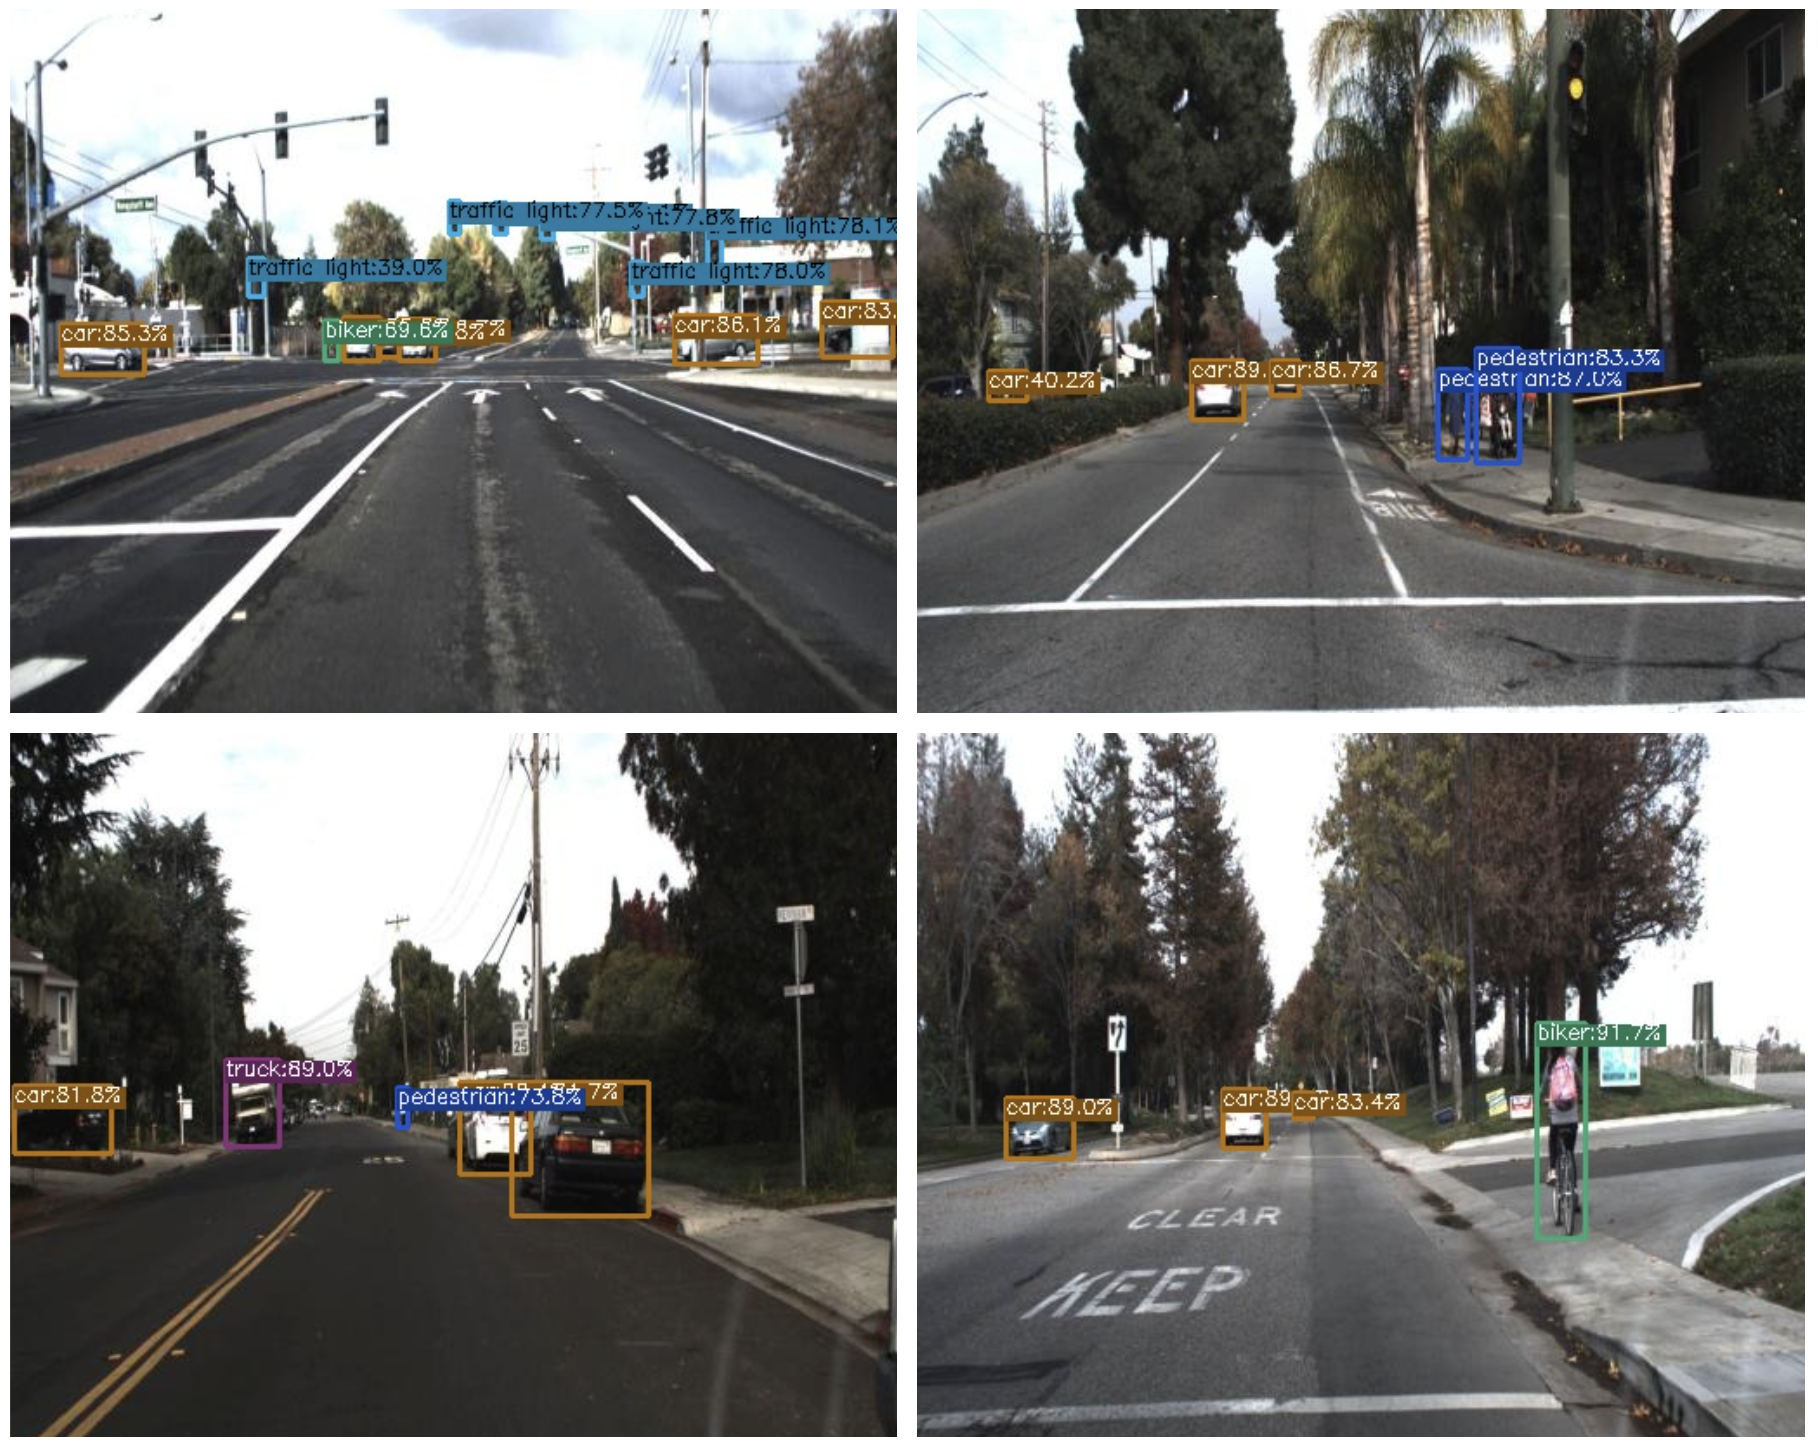
\includegraphics[width=\textwidth]{predictYOLOX.png}
	\end{subfigure}
	\hspace{0.1cm} % Anpassung des Abstands
	\begin{subfigure}[b]{0.35\textwidth}
		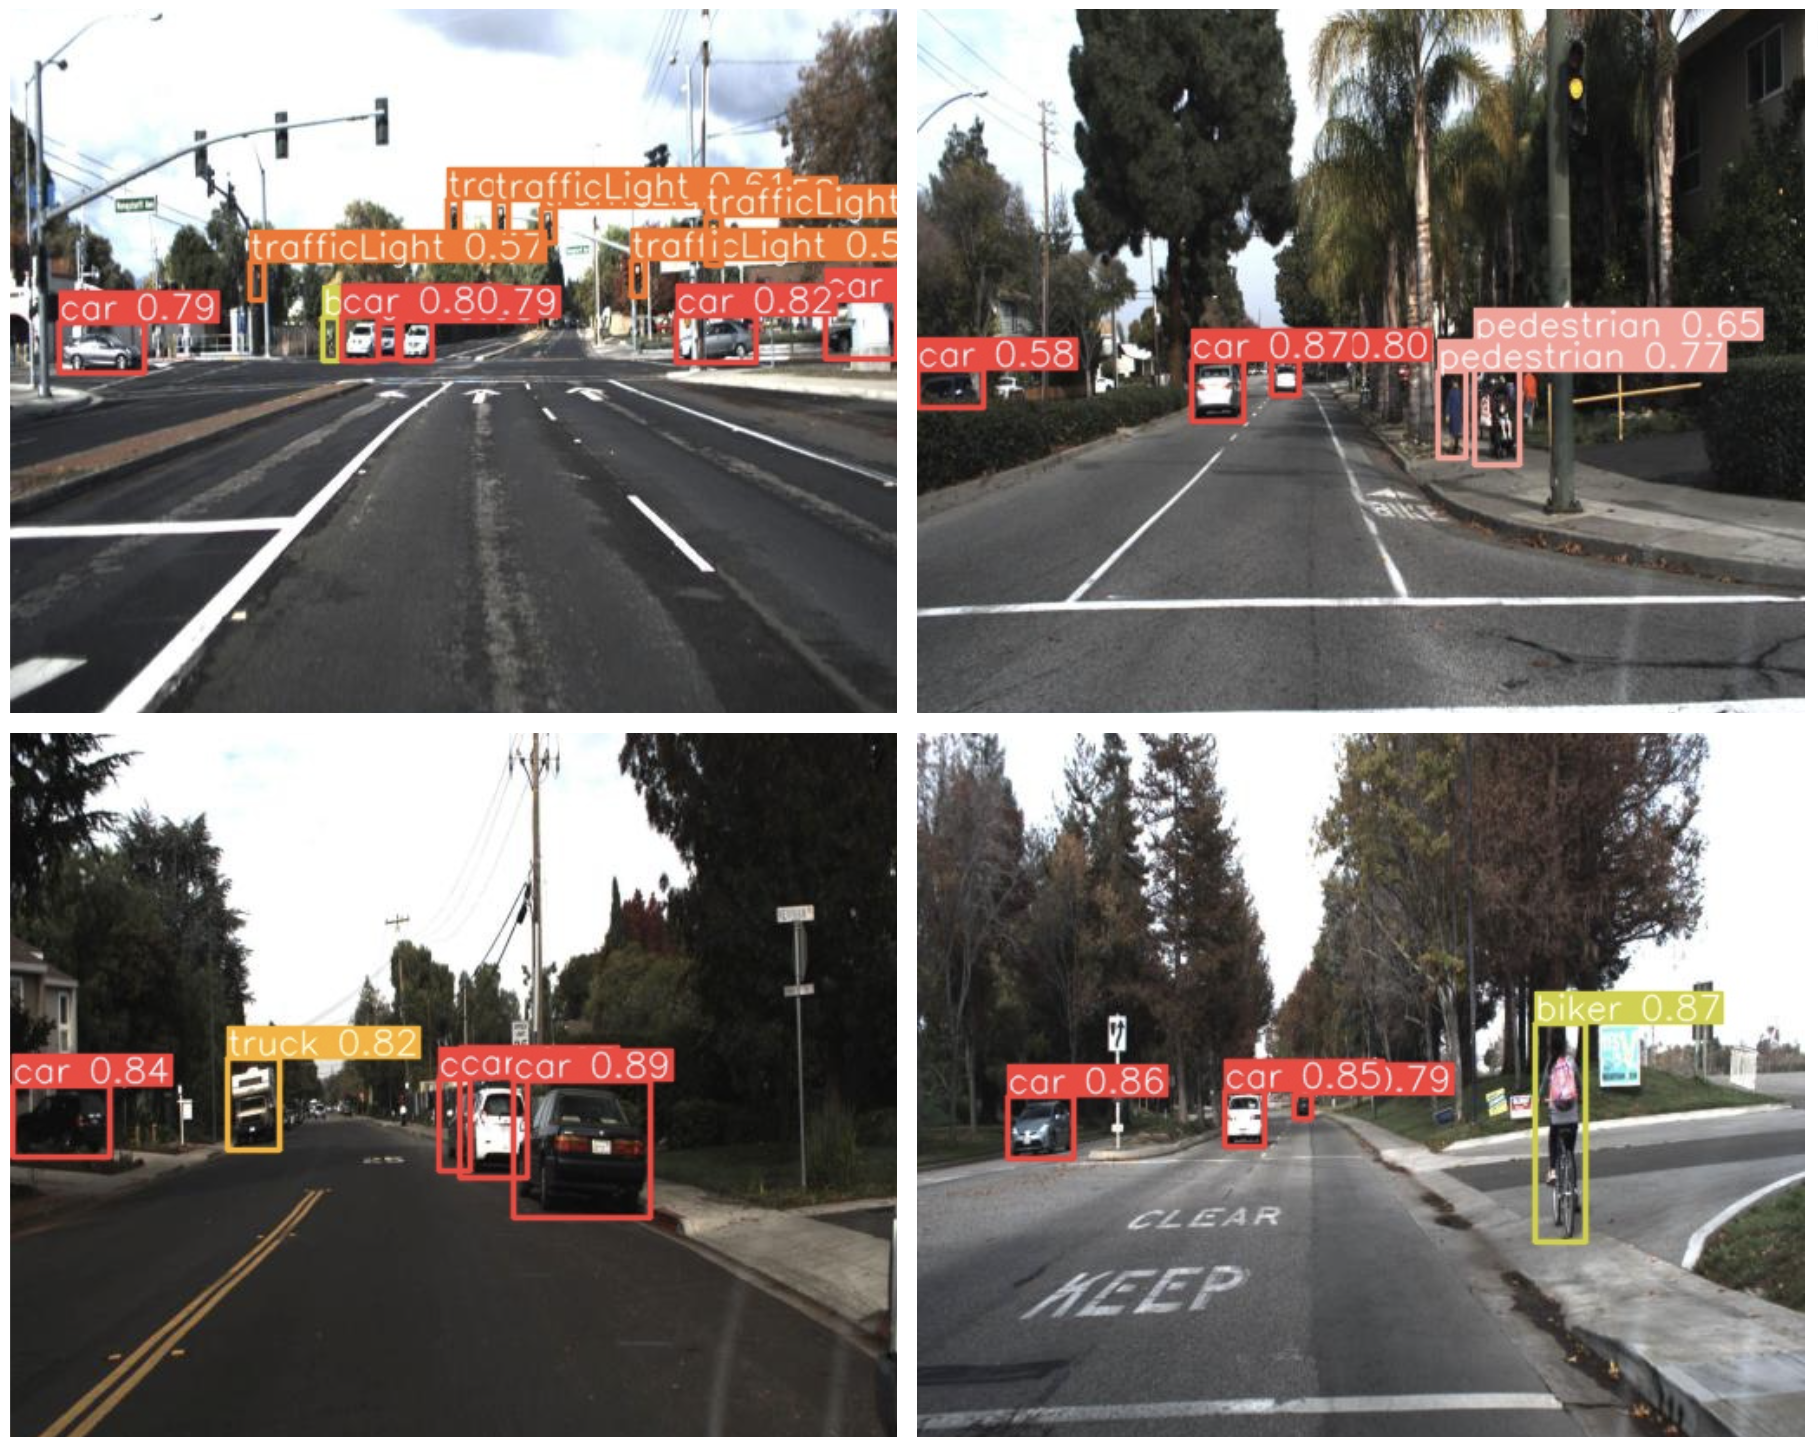
\includegraphics[width=\textwidth]{predictYOLOv8.png}
	\end{subfigure}
	\caption[Vorhersage der Netzwerke auf vier Beispielbildern aus dem Testdatensatz]{Vorhersage der Netzwerke auf vier Beispielbildern aus dem Testdatensatz. (links: YOLOX, rechts: YOLOv8) Quelle: Eigene Aufnahme}
	\label{fig:predictionNetworks}
\end{figure}


  \chapter{Zusammenfassung und Ausblick}\label{chap:conclusion}

  %\chapter{Vorlagen}

% Literaturverzeichnis \cite{label}
% Abbildungen, Tabellen, Listing, ... \autoref{label}


\section{Abbildungen}
% small h -> Latex legt fest wo Abbildung am besten liegt wegen Seitenaufteilung
% big H -> Abbildung genau an dieser stelle
\begin{figure}[h]
	\centering
	\includegraphics[width=0.55\linewidth]{sinus_plot.pdf}
	\caption[Beispiel Plot der Matplotlib Bibliothek]{Beispiel Plot der Matplotlib Bibliothek. Quelle: Eigene Aufnahme}
	\label{fig:sinus_plot}
\end{figure}


\section{Tabelle}
% l: linksbündig, c: zentriert, r: rechtsbündig
\begin{table}[H]
	\centering
	\begin{tabular}{l|c|c|c|c|c|c}
		&	Saplte 1	&	Spalte 2	&	Spalte 3	&	Spalte 4	&	Spalte 5	&	Spalte 6\\
		\hline
		Zeile 1		&	1	&	1	&	1 	&	1 &	1	&	1\\
		\hline
		Zeile 2	&	1	&	1	&	1	&	1	&	1		&	1\\
		\hline
		Zeile 3	&  1	&	1	&	1	&	1	&	1	&	1\\
		\hline
		Zeile 4	&	1	&	1	&	1	&	1	&	1	&	1
	\end{tabular}
\end{table}

\section{Programmiercode}
\lstinputlisting[caption=Matplotlib Beispiel Code. Quelle: Eigener Programmcode, label=code_Matplotlib, captionpos=b, firstline=1, lastline=11]{code/Matplotlib_Example.py}

\section{Mathematik}
\subsection{Matrix}
\begin{align}
	M =
	\begin{pmatrix}
		1 &	1	& 1 & 1\\
		1 & 1 & 1 & 1\\
		1 & 1 & 1 & 1\\
		1 & 1 & 1 & 1
	\end{pmatrix}
\end{align}


\subsection{Formel}

\begin{align}
	\begin{split}
		R(\alpha, \beta, \gamma) &=  R_z(\alpha) \cdot R_y(\beta) \cdot R_x(\gamma)\\
		&=\begin{pmatrix}
			C_\alpha\cdot C_\beta & -S_\alpha \cdot C_\gamma + C_\alpha \cdot S_\beta \cdot S_\gamma  & S_\alpha \cdot S_\gamma + C_\alpha \cdot S_\beta \cdot C_\gamma  \\
			S_\alpha\cdot C_\beta & C_\alpha\cdot C_\gamma + S_\alpha\cdot S_\beta\cdot S_\gamma & -C_\alpha\cdot S_\gamma + S_\alpha \cdot S_\beta \cdot C_\gamma \\
			-S_\beta & C_\beta \cdot S_\gamma & C_\beta \cdot C_\gamma
		\end{pmatrix}.
	\end{split}
	\label{EulerToRot}
\end{align}

\begin{equation*}
	[\bar{u}]_x \coloneqq
	\begin{pmatrix}
		0 & -\bar{u}_3 & \bar{u}_2 \\
		\bar{u}_3 & 0 & -\bar{u}_1 \\
		-\bar{u}_2 & \bar{u}_1 & 0 \\
	\end{pmatrix}
\end{equation*}

\begin{align}
	\label{VecToRot1}
	R = I + \sin(\theta)\cdot [\bar{u}]_x + (1-\cos(\theta))\cdot [\bar{u}]_x^2
\end{align}

\section{Aufzählung}
\begin{itemize}
	\item Item 1
	\item Item 2
	\item Item 3
	\item Item 4
\end{itemize}




\section{Station X: Zaun}
\subsection{Animation}
%Skirpt, Animator, Zustände zugreifen

\section{Weiteres}
%Name überlegen für Kapitel
%Animation für Igel Mutter -> von Magdalena -> Blend Tree 



  
 
  % Literaturverzeichnis
  \phantomsection
  \addcontentsline{toc}{chapter}{Literaturverzeichnis}
  \bibliographystyle{natdin}
  \bibliography{literatur}
  \newpage
  
  % Abbildungsverzeichnis
  \phantomsection
  \addcontentsline{toc}{chapter}{Abbildungsverzeichnis}
  \listoffigures
  \newpage

  % Tabellenverzeichnis
  % \phantomsection
  % \addcontentsline{toc}{chapter}{Tabellenverzeichnis}
  % \listoftables
  % \newpage
  
  %Anhang
 \chapter{Anhang}\label{chap:appendix}
\section{Ordnerstruktur}
\begin{figure}[h]
	\centering
	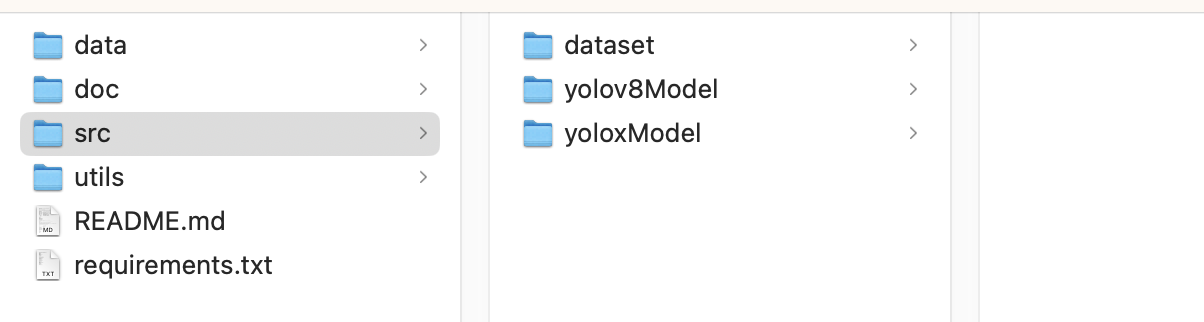
\includegraphics[width=0.55\linewidth]{folder_src.png}
	\caption[Ordnerstruktur des GitHub Repositories]{Ordnerstruktur des GitHub Repositories. Quelle: Eigne Aufnahme}
\end{figure}

\begin{itemize}
	\item data: Darin liegen die Datensätze (in GitHub nicht mit hochgeladen).
	\begin{itemize}
		\item dataFiltered: Der gefilterte Datensatz (nicht annotierte Bilder gelöscht, Klassen zusammengefügt, Train/Val/Test split) mit \textit{datasetPreprocessing.ipynb}
		\item dataRaw: Der unbearbeitete Datensatz \cite{datasetSelfDrivingCar}
		\item dataYolov8: Der Datensatz im Format für YOLOv8 mit \textit{datasetConvertion.ipynb}
		\item dataYoloX:  Der Datensatz im Format für YOLOX mit \textit{datasetConvertion.ipynb}
	\end{itemize}
	\item doc: Dort liegt die Dokumentation im LaTex-Format
	\item src: Dort liegen die Skripte (Datenvorverarbeitung, YOLOX, YOLOv8)
	\item utils: GitHub Repository von YOLOX
	\item requirements.txt: Datei für die Installation der Pakete mit \textit{pip}
\end{itemize}

\section{Dateien: Datensatz}
\begin{figure}[h]
	\centering
	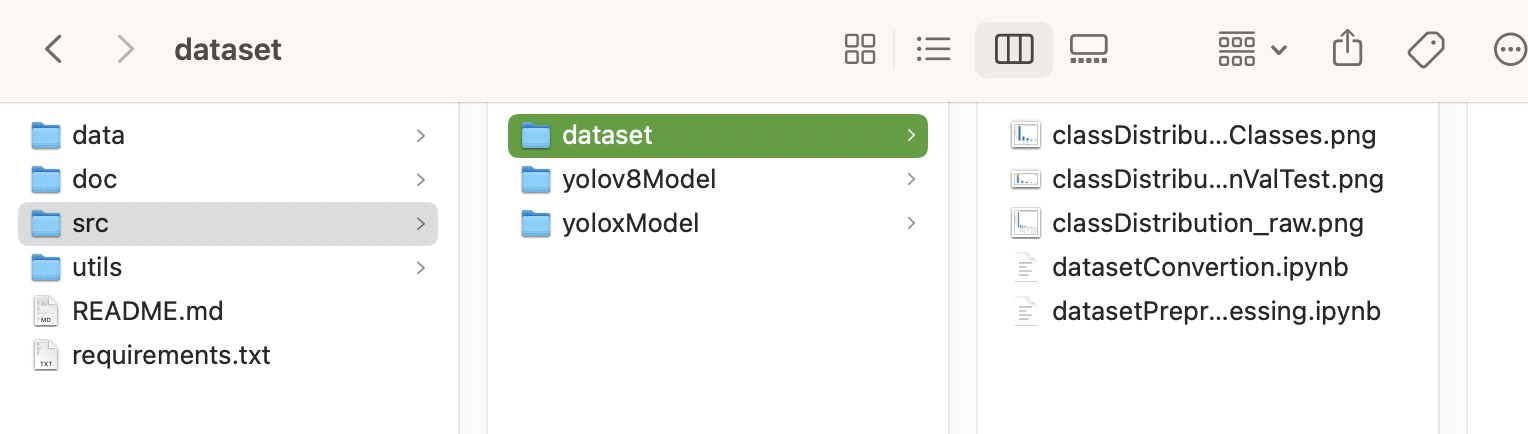
\includegraphics[width=0.55\linewidth]{folder_dataset.png}
	\caption[Ordnerstruktur des src/dataset Ordners.]{Ordnerstruktur des src/dataset Ordners. Quelle: Eigne Aufnahme}
\end{figure}

\begin{itemize}
	\item datasetConvertion.ipynb: Skript zur Umwandlung der Daten in die Formate der Netzwerke
	\item datasetPreprocessing.ipynb: Skript zur Vorverarbeitung des Datensatzes
\end{itemize}



\section{Dateien: YOLOX}
\begin{figure}[h]
	\centering
	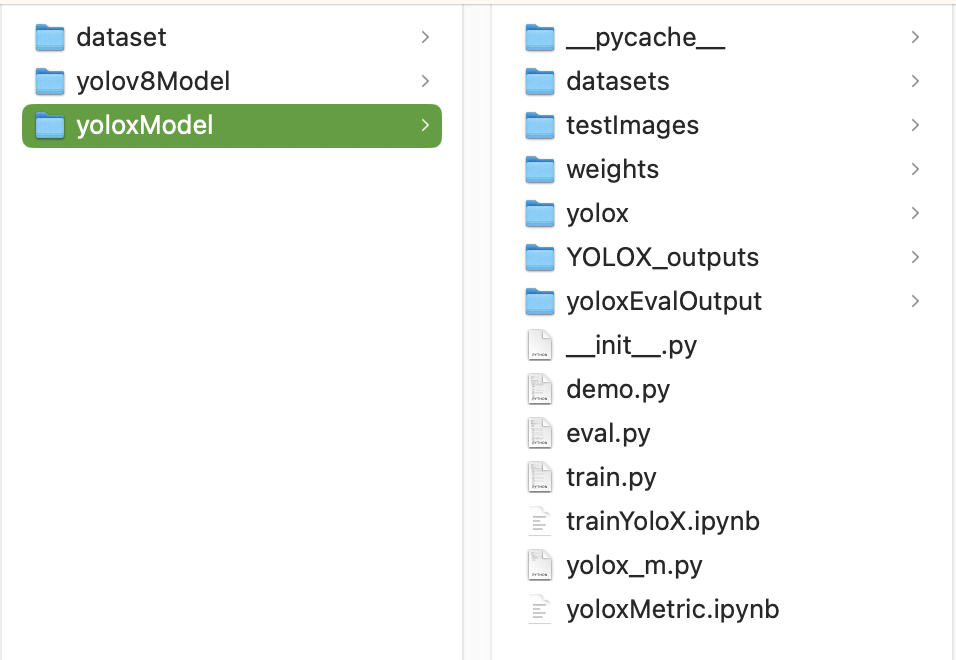
\includegraphics[width=0.55\linewidth]{folder_yolox.png}
	\caption[Ordnerstruktur des src/dataset Ordners.]{Ordnerstruktur des src/dataset Ordners. Quelle: Eigne Aufnahme}
\end{figure}

\begin{itemize}
	\item datasets: Dort liegt der Datensatz im YOLOX Format (Kopie von ./dataset/dataYoloX)
	\item testImages: Vier Testdateien aus dem Testdatensatz
	\item weights: Initialisierungsgewichte aus COCO-Training
	\item yolox: Das yolox-Netzwerk aus den GitHub Repository \cite{yoloxGitHubRepo}
	\item YOLOX\_ouputs: Ausgabe nach dem Training (Gewichte, Log, Visualisierung, ...)
	\item yoloxEvalOutput: Ausgabe im json-Format für die Evaluierung
	\item demo.py: Um das Netzwerk auszuführen auf Eingabebild (aus dem GitHub Repository \cite{yoloxGitHubRepo})
	\item eval.py: Um das Netzwerk zu evaluieren (aus dem GitHub Repository \cite{yoloxGitHubRepo})
	\item train.py: Um das Netzwerk zu trainieren (aus dem GitHub Repository \cite{yoloxGitHubRepo})
	\item trainYoloX.ipynb; Sammlung der Befehle um Netzwerk zu trainieren/evaluieren/auszuführen
	\item yolox\_m.py: Konfiguration des Netzwerks
	\item yoloxMetric.ipynb: Metriken zur Evaluierung berechnen
\end{itemize}

\section{Dateien: YOLOv8}
\begin{figure}[h]
	\centering
	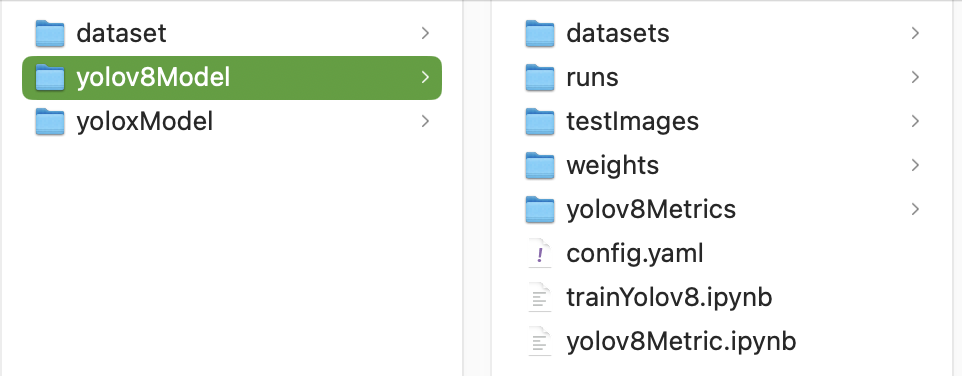
\includegraphics[width=0.55\linewidth]{folder_yolov8.png}
	\caption[Ordnerstruktur des src/dataset Ordners.]{Ordnerstruktur des src/dataset Ordners. Quelle: Eigne Aufnahme}
\end{figure}

\begin{itemize}
	\item datasets: Dort liegt der Datensatz im YOLOv8 Format (Kopie von ./dataset/dataYolov8)
	\item runs: Ausgabe nach dem Training (Gewichte, ...)
	\item testImages: Vier Testdateien aus dem Testdatensatz
	\item weights: Initialisierungsgewichte aus COCO-Training
	\item yolov8Metrics: Dateien zur Evaluierung des Netzwerks
	\item config.yaml:  Konfiguration des Netzwerks
	\item trainYolov8.ipynb: Training des Netzwerks
	\item yolov8Metric.ipynb: Metriken zur Evaluierung berechnen
\end{itemize}
\end{document}    